% ===========================================================================
% Fuel Anchoring as Reconciliation by Construction: A Greenhouse-Gas Inventory
% of Road Transport and Mixed Off-Road Mobile Combustion in Pakistan
%
% Supplementary Notes S1-S5 are a SEPARATE document: supplement.tex.
%
% Target journal: Environmental Modelling & Software (Elsevier)
% Document class: elsarticle, 5p layout
% ===========================================================================

\documentclass[5p,times,authoryear]{elsarticle}

% ===========================================================================
% Shared preamble for every manuscript in this repository.
%
% Papers using it:
%   paper/            agriculture inventory
%   paper_nowcast/    agricultural nowcasting
%   paper_national/   the nine-sector national inventory
%   notes/<sector>/   one data note per non-agriculture sector
%
% It exists because paper/ and paper_nowcast/ began as copies of one another
% and had already drifted five lines apart before a third manuscript existed.
% Eleven copies would drift eleven ways, and a macro that renders differently
% in two papers is the kind of defect nobody notices until proof stage.
%
% \graphicspath is deliberately NOT set here - each manuscript sets its own
% after \input{...preamble}, because figures live beside the document.
% ===========================================================================

\usepackage[utf8]{inputenc}
\usepackage[T1]{fontenc}
\usepackage{amsmath,amssymb}
\usepackage{graphicx}
\usepackage{booktabs}
\usepackage{multirow}
\usepackage{siunitx}
\usepackage[colorlinks=true,citecolor=blue,linkcolor=blue,urlcolor=blue]{hyperref}
% Document-information metadata for every PDF in the bundle (the seventh review noted
% the shipped PDFs carried none). Documents that set their own \hypersetup{pdftitle=...}
% keep it - hyperref takes the LAST setting, and this shared block runs first. Full
% tagged-PDF (tagpdf / \DocumentMetadata) is deliberately not attempted here: the
% installed LaTeX toolchain's support is not uniform across sixteen documents, and a
% half-tagged bundle is worse than an honestly untagged one; deferred deliberately.
\hypersetup{
  pdfauthor={Rehan Ahmad, Pakistan Air Quality Initiative (PAQI)},
  pdfsubject={A reproducible ten-sector national greenhouse-gas inventory
              for Pakistan},
  pdfkeywords={Pakistan, greenhouse gas inventory, IPCC 2006 Guidelines, MRV,
               reproducible research, emissions, air pollutants},
}
\usepackage{caption}
\captionsetup[table]{position=below}
\usepackage{enumitem}
\usepackage{xcolor}
\usepackage{float}
\usepackage{placeins}
\usepackage{tabularx}
\usepackage{natbib}
\usepackage{tikz}
\usetikzlibrary{arrows.meta,positioning,fit,backgrounds}

\setlength{\emergencystretch}{3em}

% Looser float placement to prevent pile-up in two-column mode.
\renewcommand{\topfraction}{0.95}
\renewcommand{\bottomfraction}{0.85}
\renewcommand{\textfraction}{0.05}
\renewcommand{\floatpagefraction}{0.85}
\setcounter{topnumber}{4}
\setcounter{bottomnumber}{3}
\setcounter{totalnumber}{6}

% ---------------------------------------------------------------------------
% Custom shorthand: in macros.tex since the ESSD re-targeting, because the national
% article compiles under the Copernicus class and cannot take this preamble (the class
% loads its own packages) but needs exactly the same macros. This file inputs it so that
% every other manuscript keeps compiling unchanged.
%
% THREE relative paths, because \input resolves against the COMPILE DIRECTORY and not
% against this file, so the depth is a property of whoever is building:
%   ../paper_common      a manuscript compiled from one level down
%   ../../paper_common   papers/<sector>/ and notes/<sector>/
%   ../../../paper_common  paper_national/versions/<v>/, since the national paper was
%                          versioned - that move is what added this third arm, and the
%                          supplement failed with "../../paper_common/macros.tex not
%                          found" until it was here
% A fourth depth needs a fourth arm, which is the cost of keeping a bare `latexmk` in a
% manuscript directory working without a TEXINPUTS set for it.
% ---------------------------------------------------------------------------
\IfFileExists{../paper_common/macros.tex}%
  {\input{../paper_common/macros}}%
  {\IfFileExists{../../paper_common/macros.tex}%
    {% ===========================================================================
% paper_common/macros.tex - the shorthand every manuscript shares.
%
% Split from preamble.tex in the ESSD re-targeting: the national article now compiles
% under the Copernicus class, which loads its own packages and forbids most of what
% preamble.tex sets (geometry-like options, a second hyperref, placeins), but it needs
% exactly the same shorthand as the sector reports. The macros therefore live here, on
% their own, and preamble.tex inputs this file so that every other manuscript keeps
% compiling unchanged. A macro that renders differently in two documents is the defect
% this file exists to prevent; define it once.
%
% Requires: siunitx (for \DeclareSIUnit and \si) - the caller loads it.
% ===========================================================================

% Gas and pollutant names.
\newcommand{\COtwo}{CO\textsubscript{2}}
\newcommand{\COe}{CO\textsubscript{2}e}
\newcommand{\CHfour}{CH\textsubscript{4}}
\newcommand{\NtwoO}{N\textsubscript{2}O}
\newcommand{\NHthree}{NH\textsubscript{3}}
\newcommand{\NOx}{NO\textsubscript{x}}
\newcommand{\SOtwo}{SO\textsubscript{2}}
\newcommand{\PM}{PM\textsubscript{2.5}}
\newcommand{\MCF}{MCF}
\newcommand{\Mt}{\text{Mt~\COe}}
\newcommand{\tCha}{\si{\tonne\per\hectare}}
\newcommand{\AFOLU}{AFOLU}
\newcommand{\GLW}{GLW\,4}
\newcommand{\EFone}{EF\textsubscript{1}}

% siunitx: allow Mt, Tg, ha, head, yr, dB
\DeclareSIUnit{\head}{head}
\DeclareSIUnit{\yr}{yr}
\DeclareSIUnit{\dB}{dB}

% A file name is the one long unbreakable token these documents are full of -
% \texttt{waste\_air\_pollutants\_2024.csv} is wider than a two-column measure and TeX prints
% it past the margin rather than breaking it. Allowing a break AFTER each escaped underscore
% costs nothing and inserts no hyphen, which matters: a hyphenated file name is a wrong file
% name. This is one line because every such name in every document is written with \_.
\let\pkinvunderscore\_
\renewcommand{\_}{\pkinvunderscore\allowbreak}
}%
    {\input{../../../paper_common/macros}}}
% Long unbreakable strings - output filenames, module paths, URLs in \texttt - do not fit a
% two-column measure and TeX prints them past the margin rather than breaking them. Nothing
% read the log, so 47 of those overruns shipped across seven documents. Emergency stretch lets
% the paragraph loosen instead, and \texttt is taught to break at the punctuation these names
% actually contain.
\emergencystretch=6em


\graphicspath{{figures/}}

% ---------------------------------------------------------------------------
\journal{Environmental Modelling \& Software}
% ---------------------------------------------------------------------------

\begin{document}

\begin{frontmatter}

\title{PakEmis Sector Technical Note TN03\\[4pt]
Fuel Anchoring as Reconciliation by Construction: A Greenhouse-Gas Inventory of
Road Transport and Mixed Off-Road Mobile Combustion in Pakistan}

\author[paqi]{Rehan Ahmad\corref{cor1}}
\ead{rehan@pakairquality.com}

\address[paqi]{Pakistan Air Quality Initiative (PAQI), Karachi, Pakistan}

\cortext[cor1]{Corresponding author}

% --- Abstract ---
\begin{abstract}
Transport inventories are usually built bottom-up from a vehicle fleet and reconciled
against fuel supply afterwards, resting their weakest input---fleet activity---under their
most-used output. We invert that for Pakistan: road transport (IPCC 1A3b) and mixed
off-road machinery are anchored on the road customer class of OCAC's sectoral petroleum
sales for FY2023--24 (\SI{7209}{\kilo\tonne} petrol, \SI{5551}{\kilo\tonne} diesel; those
customer classes sum to the national total exactly, excluding bulk industrial, utility,
government and railway diesel by construction) and on metered transport CNG. The fleet
model distributes this fuel and cannot size it: a bottom-up build on the same data would
miss diesel by half and overstate CNG threefold. Class shares are vehicle-kilometres
weighted by declared energy intensities and normalised within each fuel, so that judgement
moves composition and never magnitude---correcting it from distance-only weighting moved
two-wheelers from \SI{42.3}{} to \SI{34.1}{\percent} of on-road \COtwo{}
(\SI{13.40}{\mega\tonne}) while the sector total
moved by \SI{0.05}{\mega\tonne}. We report \SI{40.19}{\mega\tonne}~\COe{} as the
\emph{conditional road residual under the current claimant assignment} and
\SI{1.73}{\mega\tonne} for mixed off-road machinery, with a two-tier ledger that closes
both controls exactly and carries the unresolved retail-channel claimants as status rows,
priced at 2.5--10\% of the road row and treated as transfers to other IPCC categories
rather than reductions. An independent railway cross-check agrees to \SI{3.8}{\percent},
and against a fiscal-year-blended EDGAR benchmark the estimate is \num{0.85} of
it---a scope-approximate diagnostic, since EDGAR's transport boundary is inferred
rather than published. The
reported interval is $\pm\SI{11.4}{\percent}$, conditional on the boundary; a ten-year
fuel-based series and per-fuel provincial allocations follow at no further modelling cost.

\end{abstract}

\begin{keyword}
road transport emissions \sep fuel-based inventory \sep off-road machinery \sep
vehicle fleet model \sep emission factor tables \sep control total \sep
air pollutants \sep IPCC 2006 Guidelines \sep Pakistan \sep MRV
\end{keyword}

\end{frontmatter}

%% Generated by scripts/make_release_cover.py; says which release this documents.
% The Sector Technical Note banner (v1.0.0). Each sector manuscript is a PakEmis Sector
% Technical Note, numbered TN01-TN10 in src/pkinv/release.py (TECHNICAL_NOTES), and says
% so on its first page: it documents ONE sector module of the release named in the block
% that follows, and the national totals are stated only in the data-description article
% (the cover block below reproduces them as release identity, not as a claim of this note).
% Usage, in the document body before the release cover:  \TNBanner{TN01}
\providecommand{\TNBanner}[1]{%
  \noindent\fbox{\parbox{\dimexpr\linewidth-2\fboxsep-2\fboxrule}{%
    \textbf{PakEmis Sector Technical Note #1.} Technical documentation of one sector
    module of the PakEmis release identified below, deposited with the data as part of the
    documentation record. The national data-description article (\texttt{paper\_national/})
    is the only document that states the national totals as its own result.%
    \InputIfFileExists{../../paper_common/generated_availability_tn}{}{}%
  }}\par\medskip}

\TNBanner{TN03}
%% GENERATED by scripts/make_release_cover.py from outputs/release_manifest.json.
%% Do not edit: the edit will be overwritten and CI diffs the result.
\newcommand{\ReleaseCover}{%
\begin{center}\small
\setlength{\fboxsep}{4pt}%
\fbox{\begin{minipage}{\dimexpr\linewidth-2\fboxsep-2\fboxrule\relax}\footnotesize
\textbf{Release provenance.} This document describes PakEmis under the period, configuration and source boundaries specified in its methods. The identifiers below link it to the accompanying products and source register.\\[2pt]
\begin{tabular}{@{}p{0.32\linewidth}@{\hspace{0.03\linewidth}}p{0.65\linewidth}@{}}
Release version & \texttt{1.0.0rc69} \\
Commit & \texttt{d8d874622f9a} \\
Reporting period & July 2015--June 2025 (ten fiscal years) (2015-07-01 to 2025-06-30) \\
Reference & S\_TAN (household survey; TAN nitrogen) \\
FY2023--24 total & 444.61 Mt \COe{} (AR5) under S\_TAN, the reference; 449.85 Mt under L\_TAN \\
Release manifest & \texttt{ac0ffe93ad9fcd88} (SHA-256 of \texttt{outputs/release\_manifest.json}, first 16) \\
Source manifest & \texttt{c1be6d314cfce1ea} (SHA-256 of \texttt{data/manifests/source\_manifest.csv}, first 16) \\
Data-description article & \texttt{paper\_national/} (ESSD, in preparation), same release
\end{tabular}
\end{minipage}}
\end{center}}

\ReleaseCover

% ---------------------------------------------------------------------------
% Main body
% ---------------------------------------------------------------------------

% ===========================================================================
\section{Introduction}
\label{sec:introduction}
% ===========================================================================

There are two ways to build a road transport inventory and they fail differently.

The bottom-up approach estimates the vehicle fleet, assigns annual kilometres and fuel economy
by class, and sums. It produces a rich result---emissions by vehicle type, useful for
projecting the effect of a fleet policy---and a fuel demand that will not match the national
petroleum supply. The compiler then adjusts something until it does.

The fuel-anchored approach starts from the supply figure and distributes it across classes.
It produces a total that matches national statistics by construction and a composition that is
only as good as the fleet model. Nothing needs reconciling because nothing was independently
estimated.

Which is better depends on which number is more trustworthy. In Pakistan that is not close:
the petroleum supply figure is a metered, taxed, nationally reported quantity, while the
vehicle fleet is a registration database that counts vehicles administratively rather than
by where they operate, includes a residual catch-all class, and says nothing about how far
each is driven. This paper quantifies the gap directly: the bottom-up fuel demand the same
fleet data imply, under declared engineering intensity bands, misses the observed diesel
control by half and overstates metered CNG threefold
(Section~\ref{sec:validation})---errors in both directions, which is the strongest form
of the case for letting fuel set the magnitude.

\subsection{What this paper does}

We report Pakistan's road transport and off-road mobile machinery for FY2023--24 on the
fuel-anchored basis, and treat the consequences of that choice as the subject rather than as
an implementation detail.

The consequence that matters most is that anchoring makes a boundary problem explicit.
Pakistan's petroleum statistics do publish a sectoral split---OCAC's customer-class sales
tables, which this edition anchors on directly---but a customer class is a sales channel,
not an end use: the retail Road row still contains diesel bought at pumps for stationary
agricultural plant and captive generators. This paper reads the observed customer-class
partition into a two-tier fuel-claimant ledger, carves out what a sibling sector measures
(household-generator petrol), partitions off-road machinery, cross-checks the rail
boundary against an independent source, and states plainly what remains inside the road
residual and in which direction it biases the result.

\subsection{Why Pakistan, and why anchoring in particular}

Pakistan's most recent full national inventory submission reports for FY2017--18
\citep{pakbur1}, and the international products that fill the gap must be compared with the
years matched, because Pakistan's fuel demand moved sharply after 2022. On a scope
inferred from EDGAR's category-resolved Pakistani source files---road, rail and civil
aviation---this inventory's corresponding construction is \num{0.85} of EDGAR's
fiscal-year blend of \SI{48.13}{\mega\tonne} \citep{edgar2025booklet}
(Section~\ref{sec:validation}), sitting \emph{under} the benchmark for the reasons the
customer-class boundary predicts. The blend is half of EDGAR's 2023 column and half of
its 2024 one, because this sector's July--June reference period falls across both; the
comparison is a scope-approximate diagnostic rather than a validation, because EDGAR's
transport boundary is inferred rather than published.

Anchoring is particularly appropriate here for a reason specific to the country's fleet.
Two-wheelers are the largest single class in Pakistan's road transport---under the
reference allocation they receive \SI{13.40}{\mega\tonne}, \SI{34.1}{\percent} of
on-road \COtwo{}---and their annual kilometres are among the least well-constrained
inputs in this Pakistani fleet model. A bottom-up estimate would rest a very large term on
one of its weakest inputs. Anchored, that same uncertainty affects only how the fuel is
split between classes, which is exactly what happened when this edition corrected the
split: two-wheelers fell by six megatonnes, heavy diesel rose past them, and the sector
total moved by \SI{0.05}{\mega\tonne} (Section~\ref{sec:results}).

\subsection{Contributions}

\begin{enumerate}[leftmargin=*,itemsep=2pt,topsep=3pt]
\item \textbf{A fuel-anchored road transport inventory for Pakistan} anchored on the
  customer-class rows of the national sectoral sales table, so the sector total
  reconciles with petroleum statistics by construction and the bulk non-road claimants
  are excluded by the source's own structure (Section~\ref{sec:methods}).
\item \textbf{A two-tier fuel-claimant ledger, mostly observed}: the national tier is
  OCAC's own exhaustive customer-class partition; the road tier carries one relayed
  carve-out (generator petrol, closed against the residential module), one partition
  (off-road machinery), an independent rail cross-check between two unrelated sources,
  and the unresolved retail claimants as bounded status rows instead of silence
  (Table~\ref{tab:ledger}).
\item \textbf{A quantified instance of the IPCC parallel-table trap}, in which the plausible
  wrong table leaves \COtwo{} exactly right and moves the category by \SI{8}{\percent} through
  \NtwoO{} alone---invisible to every \COtwo{}-dominated comparison available
  (Section~\ref{sec:factors}).
\item \textbf{A source-traceable road air-pollutant estimate} using EMEP/EEA Tier~1 fuel-based exhaust factors, which the guidebook derives from its hot and cold Tier~3 method for a typical 2010 EU-27 fleet (no Pakistan-specific cold-start treatment is applied), separate petrol evaporation and tyre/brake/road-surface wear. Transferred fleet factors, technology, sulfur compliance and resuspended road dust retain their actual limitations (Section~\ref{sec:air}).
\item \textbf{A provincial petroleum allocation from OCAC's monthly area editions},
  allocated per fuel, with a published diagnostic demonstrating the failure of the
  registration proxy it replaces and an allocation crosswalk stating which streams ride
  which proxy (Section~\ref{sec:results}).
\end{enumerate}

Method shared with the other nine sectors of the national inventory---the module contract,
the accounting closures, the parameter-uncertainty treatment---is documented separately
\citep{ahmad2026national} and not repeated here.

% ===========================================================================
\section{Related Work}
\label{sec:related}
% ===========================================================================

\subsection{Fuel-based and fleet-based transport inventories}

The IPCC 2006 Guidelines describe both approaches for 1A3b and are explicit that the fuel-based
Tier~1 is preferred where national fuel statistics are reliable and fleet data are not
\citep{ipcc2006energy}. That guidance is often inverted in practice, because a fleet-based estimate
produces the disaggregation that transport policy wants and a fuel-based one does not.

The position taken here is that the two are not alternatives at the same level. The fuel
figure determines the total; the fleet model determines the split. Running the fleet model
\emph{inside} the fuel constraint gives the policy-relevant disaggregation without letting it
set the magnitude, which is the arrangement the guidelines' preference implies but which is
rarely stated as such.

\subsection{Global products and their transport scope}

EDGAR \citep{edgar2025booklet,crippa2020} reports Pakistani transport across all modes---road, rail,
domestic aviation and navigation together. Comparing that against a road-only estimate is a
scope error that will make any road inventory look low; Section~\ref{sec:validation} walks
the scope component by component instead, and labels the result honestly as fiscal-year blended
and partially scope-harmonized.

Climate TRACE \citep{climatetrace} constructs road transport from asset and activity
inference. Both are global models applying globally consistent assumptions, which is their
strength across countries and their limitation within one: neither can know that Pakistan's
national diesel figure includes agricultural and captive-generation fuel, which is the single
largest scope question in this sector.

\subsection{Off-road machinery, and where it belongs}

IPCC reports off-road mobile machinery outside road transport, and not all under one
category: agricultural tractors and plant go to 1A4c\,ii, while construction and industrial
machinery belongs under 1A2 (manufacturing and construction, gvii). This is easy to state
and easy to get wrong in a country where the diesel that runs all of it comes from the same
retail pumps as the diesel that runs the trucks and is not separately reported---and this
inventory gets it only partly right: its off-road class inherits a residual bucket that
mixes both, and is reported under the mixture-declaring name \emph{Mixed off-road
(1A4c/1A2)} with the misassignment declared in the completeness table and priced as a
reporting-recode scenario rather than resolved (Section~\ref{sec:limitations}).

The usual treatments are to leave it inside road transport, which overstates 1A3b and leaves
1A4c empty, or to estimate it separately from a machinery population, which double-counts the
fuel unless the road control total is reduced correspondingly. Section~\ref{sec:methods}
describes a third: carve it out of the same control total by vehicle-kilometre share, so the
two categories partition one quantity of diesel.

\subsection{The parallel-table problem}

Chapter~3 of Volume~2 publishes separate default tables for road, rail and off-road mobile
sources, and the same diesel appears in all of them with identical \COtwo{} and sharply
different \NtwoO{}. The distinction reflects real combustion differences---catalyst-equipped
road engines against uncontrolled off-road ones---but the tables are easy to conflate because
the fuel is bought from the same pump.

The national manuscript documents four instances of this trap across the inventory
\citep{ahmad2026national}. Section~\ref{sec:factors} treats the one that arises here, and
reports the diagnostic the engine emits on every run so the consequence is a number rather
than a caution.

% ===========================================================================
\section{Study Area and Data}
\label{sec:data}
% ===========================================================================

\subsection{The control totals}

The petroleum activity data are the \emph{Road} customer-class rows of OCAC's Sectoral
Sales of Energy Products for FY2023--24 \citep{ocacarchive}---the sector's reference
period under the same July--June fiscal convention the CNG stream pins by test. OCAC publishes
this table as sector rows (Domestic, Industry, Agriculture, Transport---itself split into
Road, Railways, Domestic Bunkers and two aviation rows---Power, Government) by product
columns in tonnes, and the customer classes sum to the printed national total exactly.
Road is a \emph{customer class}: retail pump sales. Bulk industrial, utility, government
and railway diesel never enters it, so those claimants are excluded from the road control
by construction rather than carved out of it.

\begin{table}[htbp]
\centering
\footnotesize
\begin{tabular}{@{}lrr@{}}
\toprule
\textbf{Fuel} & \textbf{TJ} & \textbf{Share (\%)} \\
\midrule
Petrol & 316\,882 & 57.0 \\
Diesel & 238\,712 & 43.0 \\
\midrule
\textbf{Total} & \textbf{555\,594} & \textbf{100.0} \\
\bottomrule
\end{tabular}
\caption{The petroleum road controls for FY2023--24: the OCAC Road rows (petrol = MS + HOBC,
\SI{7209}{\kilo\tonne}; diesel \SI{5551}{\kilo\tonne}) converted at IPCC net calorific
values. CNG is a third, separately controlled activity basis (Section~\ref{sec:methods})
and does not appear here because it is not petroleum. The full claimant structure over
these controls is Table~\ref{tab:ledger}.}
\label{tab:fuel}
\end{table}

\begin{figure*}[htbp]
\centering
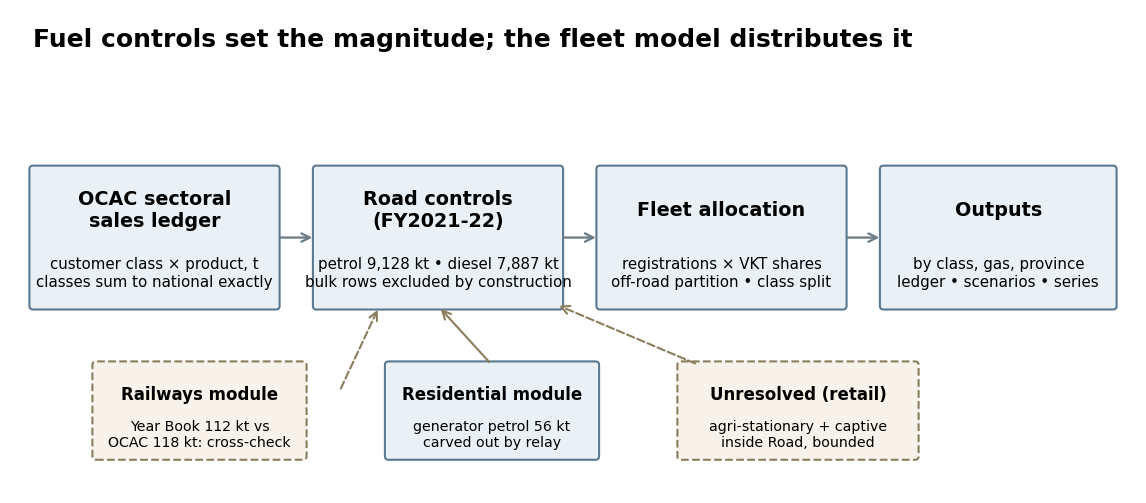
\includegraphics[width=0.92\linewidth]{transport_framework.png}
\caption{The calculation, end to end: the OCAC customer-class ledger supplies the road
controls, the fleet model distributes them, and the cross-sector relays (railways as a
cross-check, residential as a carve-out) and the unresolved retail claimants are explicit
boxes rather than prose. The high petrol share of the controls is consistent with
Pakistan's large two-wheeler fleet.}
\label{fig:activity}
\end{figure*}

\subsection{A provenance audit: the superseded control}

The previous edition anchored on national supply figures derived from the Economic
Survey's provisional nine-month FY2025 data. Those stored values---\SI{10162}{} and
\SI{8820}{\kilo\tonne}---were arithmetically inconsistent with their own source note: they
equal the nine-month figures times $16/9$, not the documented $12/9$ annualisation, an
annualisation applied twice. The diesel figure coincidentally landed within one percent of
the FY2021--22 \emph{national} internal HSD total, so the matched-year EDGAR comparison
looked right on a wrong-provenance number; the petrol figure overshot the fiscal-year
national total by eleven percent. A match against a benchmark is not provenance. The
superseded pair is retained as a named, executable boundary scenario
(\texttt{legacy\_pes\_control}, Section~\ref{sec:results}) rather than deleted---the same
discipline the residential sector applies to its superseded dung basis---so the bridge
from previously published numbers stays open and honest.

\subsection{What the road rows still include that they should not}

A customer class cannot see end uses. Retail pumps sell diesel to trucks, but also to
tube-well and thresher owners (stationary agriculture, IPCC 1A4c~i) and to captive
generator operators (1A2); retail petrol includes fuel carried home for household
generators (1A4b). One of these three is carved out---the generator petrol, relayed from
the residential module (Section~\ref{sec:methods})---and the two diesel claimants remain
inside, unresolved, biasing the road residual high conditional on the other deductions.
Two observations frame them: OCAC books \emph{zero} bulk HSD to its Agriculture row in
all ten editions, so the agricultural claim is retail-channel only; and the road share
of national diesel spans 0.83--0.91 across the ten-year panel---a customer-class
boundary sensitivity that bounds the sales channel, not the contamination within it,
which is priced separately by the retail non-road scenarios of
Section~\ref{sec:results}. The complete claimant
structure---observed bulk rows, carve-outs, residuals and unresolved status rows---is
the two-tier fuel ledger of Table~\ref{tab:ledger}.

\subsection{The fleet model}

Vehicle classes and their shares come from the national registration statistics
\citep{provregstats}, which give counts by class and province. Annual vehicle-kilometres
and fuel-split shares by class come from the transport parameter table, whose survival
parameters derive from a district-level Punjab transport manuscript \citep{naveedpunjab}
that adopts the survival functions of \citet{guttikunda2024}.

The classes are two- and three-wheelers, four-wheelers in three size bands, light and heavy
duty vehicles, buses, and an off-road class. That last one is a genuine complication rather
than a clean category, and Section~\ref{sec:limitations} treats it: the source workbook maps
its catch-all "other vehicles" entry into off-road wholesale, so the class is a residual as
well as a machinery category, and it is reported under the mixture-declaring name
\emph{Mixed off-road (1A4c/1A2)}.

\subsection{Air-pollutant factors}

The exploratory air-pollutant diagnostic (\ref{sec:air}) applies per-kilometre
factors to the same survival-weighted vehicle-kilometres that distribute the fuel control
total. The factors are transcriptions from the Punjab emissions workbook, and carry no
primary citation---the source file has no provenance column, and no published provenance
for them has been located here. They are consistent in magnitude with European
exhaust-factor compilations, but that is a plausibility observation, not a citation, and
it is why the layer is reported as an appendix diagnostic with no policy weight
(Section~\ref{sec:limitations}). NMVOC is non-methane VOC and \NOx{} is reported as
NO$_2$-equivalent mass, the inventory-wide basis.

\subsection{What this inventory had not read}

Pakistan publishes no nationally representative vehicle-kilometre survey that this study
could identify, and no on-road fuel-economy measurement was found. Everything else this
sector once described as unobtained turned out to be a reading failure, twice.

Compressed natural gas was the first instance: a substantial CNG fleet whose fuel sits in
the gas statistics, absent from the sector entirely while the transport row of OGRA's
sector-wise gas consumption table---the same table this inventory already read for the
residential control total---sat unread \citep{ogra2024,ograarchive}. That row became the
sector's third fuel control, and the previous edition drew the lesson: not absent, unread.

The OCAC sectoral tables are the second instance, at larger stakes, and the lesson applied
to the sentence that drew it. Two editions of this paper described OCAC's product-by-sector
sales as published but not obtained here. They were in the repository throughout---forty-eight monthly editions carrying
CUMULATIVE national tables, fetched by the aviation sector for their jet-fuel columns,
indexed, hashed, and already read by the residential sector for a kerosene cell; a
distinct population from the thirty-six DIRECT single-month editions below, as the edition
inventory (\texttt{outputs/ocac\_edition\_inventory.csv}) now distinguishes. This edition anchors on them (Section~\ref{sec:methods}) and builds its provincial
allocation from area pages (Section~\ref{sec:results}). There is now a third episode of
the same lesson: an earlier edition borrowed FY2024--25's provincial shape on the claim
that the reference year's area pages were never published, while the thirty-six direct
monthly editions carrying them sat fetched and hash-pinned in the repository. All three
episodes are kept here, in the data section, as the clearest available statement of what
``not obtained'' usually means in practice.

% ===========================================================================
\section{Methods}
\label{sec:methods}
% ===========================================================================

\subsection{Anchoring: the fleet distributes, it does not size}

Emissions for gas $g$ from class $c$ burning fuel $f$ are
\begin{equation}
E_{g,c,f} \;=\; A_f \cdot s_{c,f} \cdot EF_{g,f},
\end{equation}
where $A_f$ is the road-class supply of fuel $f$ in terajoules, $EF_{g,f}$ the IPCC default
factor, and $s_{c,f}$ the share of that fuel attributed to class $c$. The shares are
normalised energy products,
\begin{equation}
s_{c,f} \;=\; \frac{N_c \, k_c \, q_{c,f} \, e_{c,f}}
                   {\sum_{c'} N_{c'} k_{c'} q_{c',f} e_{c',f}},
\end{equation}
over vehicle counts $N$, annual kilometres $k$, the fraction $q$ of a class's travel on
fuel $f$, and the per-kilometre energy intensity $e$ in megajoules. The intensities are
\emph{declared engineering judgement}---generic band midpoints recorded per class and
fuel in the parameter table, not Pakistani measurements, and the same values the
fleet-implied fuel diagnostic of Section~\ref{sec:fuelgap} uses.

Because the shares are normalised, $\sum_c s_{c,f} = 1$ by construction, and therefore
$\sum_c E_{g,c,f} = A_f \cdot EF_{g,f}$ regardless of what the fleet model says. The sector
total is a function of the fuel controls and the IPCC factors alone.

That normalisation is also what bounds the declared intensities. No choice of $e$ can
move a control total or the sector magnitude; it moves \emph{composition}, and---through
the off-road partition, which is one cell of the same normalisation---which IPCC
category carries a fixed quantity of diesel. Both consequences are priced as scenarios
in Section~\ref{sec:results} rather than folded into an interval. Admitting a judgement
into the calculation at all is a real cost, and it is paid where it does least damage:
a quantity nobody has measured determines which class is said to have burnt the fuel,
never how much fuel there was.

The previous edition of this paper printed the equation above with $e$ in it while the
code applied $e \equiv 1$---normalising distance alone, which asserts that a
motorcycle-kilometre burns as much petrol as a car-kilometre and a van-kilometre as much
diesel as a truck-kilometre. Neither is true, and the correction is not small: the
two-wheeler share of the petrol control falls from 0.8119 on distance alone to 0.6100 and the class that
dominates on-road \COtwo{} changes (Section~\ref{sec:results}). The equation and the
engine now agree, and a test recomputes both normalisations from the parameter files to
assert which one the published weights came from.

This is the property that makes the fleet model's weaknesses tolerable. An error in
two-wheeler annual kilometres moves fuel between two-wheelers and everything else; it does not
change how much fuel the road class bought. The estimate that policy uses for the national
total is therefore insulated from the input that a bottom-up inventory would rest it on.

Unless stated otherwise, every $\pm$ figure in this paper and its supplement is an
approximate \SI{95}{\percent} relative half-width: IPCC Approach~1 propagation where a
value is quoted for a category or the sector, and the 2.5th--97.5th percentile band of
the Monte Carlo where a result is labelled as such.

\subsection{The fuel ledger: two carve-outs' worth of structure, mostly observed}
\label{sec:ledger}

The previous edition partitioned a national supply figure by argument---carve this out,
declare that unresolved. Anchoring on the OCAC customer-class rows turns most of that
argument into observation: the national tier of the ledger is OCAC's own partition, whose
classes sum to the printed national total exactly, and only the road tier still needs
carve-outs and status rows. Table~\ref{tab:ledger} is the complete structure; the engine
writes it on every run and aborts if any of the four (fuel, tier) ledgers fails to close.

\begin{table*}[htbp]
\centering
\scriptsize
\begin{tabular}{@{}llllrr@{}}
\toprule
\textbf{Fuel} & \textbf{Tier} & \textbf{Claimant} & \textbf{IPCC} & \textbf{kt} &
\textbf{Share} \\
\midrule
Diesel & national & National internal HSD sales (opening) &  & 6\,234.2 & 1.000 \\
Diesel & national & Domestic & 1A4b & 0.0 & 0.000 \\
Diesel & national & Agriculture (bulk) & 1A4c\,i & 0.0 & 0.000 \\
Diesel & national & Industry (incl.\ bulk captive) & 1A2 & 400.4 & 0.064 \\
Diesel & national & Railways & 1A3c & 107.9 & 0.017 \\
Diesel & national & Domestic bunkers (navigation) & 1A3d & 3.1 & 0.000 \\
Diesel & national & Power (utility) & 1A1a &  41.1 & 0.007 \\
Diesel & national & Government & various & 130.3 & 0.021 \\
Diesel & national & \textbf{Road (retail pump sales)} & 1A3b & \textbf{5\,551.4} & 0.890 \\
\midrule
Diesel & road & Off-road machinery partition & 1A4c\,ii/1A2\,gvii & 492.5 & 0.089 \\
Diesel & road & \textbf{On-road residual} & 1A3b & \textbf{5\,059.0} & 0.911 \\
Diesel & road & Stationary agricultural plant (retail) & 1A4c\,i &
  \multicolumn{2}{c}{unresolved here} \\
Diesel & road & Captive generation (retail) & 1A2 &
  \multicolumn{2}{c}{unresolved here} \\
Diesel & road & Other retail stationary/non-road uses & various &
  \multicolumn{2}{c}{unresolved here} \\
\midrule
Petrol & national & National internal MS+HOBC sales (opening) &  & 7\,252.0 & 1.000 \\
Petrol & national & Industry & 1A2 & 25.7 & 0.004 \\
Petrol & national & Government & various & 16.9 & 0.002 \\
Petrol & national & \textbf{Road (retail pump sales)} & 1A3b & \textbf{7\,209.4} & 0.994 \\
\midrule
Petrol & road & Household generators (carve-out) & 1A4b & 56.3 & 0.008 \\
Petrol & road & \textbf{On-road residual} & 1A3b & \textbf{7\,153.1} & 0.992 \\
\bottomrule
\end{tabular}
\caption{The two-tier fuel-claimant ledger, FY2023--24
(\texttt{outputs/transport\_fuel\_ledger\_2024.csv}). National-tier rows are OCAC's own
customer classes---observed, not argued---and close to the printed national totals
exactly. Road-tier unresolved rows carry no quantity by design: the on-road residual is
biased high by them, conditional on the other deductions. The third unresolved row exists
because the named claimants are not proven exhaustive within pump sales; the retail
non-road scenarios of Table~\ref{tab:boundary} price the whole within-channel claim at
2.5--10\%. The ten-year road share of national diesel (0.83--0.91) is a customer-class
boundary sensitivity---it bounds the sales channel, not the contamination within it.
Closure is an arithmetic property of the ledger, not evidence that the residual is road;
the evidence for the residual's composition is the customer-class semantics of the Road
row, and its remaining contamination is these rows, never silence.}
\label{tab:ledger}
\end{table*}

The ledger closes in mass. What it does not show is the step from mass to the energy
the engine actually distributes, and that step is not symmetric between the two fuels:
Table~\ref{tab:fuelbridge} makes it explicit.

\begin{table}[htbp]
\centering
\footnotesize
\begin{tabular}{@{}llrr@{}}
\toprule
\textbf{Fuel} & \textbf{Step} & \textbf{kt} & \textbf{TJ} \\
\midrule
Petrol & OCAC Road row (MS+HOBC)   & 7\,209.4 & 319\,377 \\
Petrol & less household generators & $-$56.3  & $-$2\,495 \\
Petrol & \textbf{operative control} & \textbf{7\,153.1} & \textbf{316\,882} \\
\midrule
Diesel & OCAC Road row (HSD)       & 5\,551.4 & 238\,712 \\
Diesel & less off-road partition   & $-$492.5 & $-$21\,177 \\
Diesel & \textbf{operative on-road control} & \textbf{5\,059.0} & \textbf{217\,535} \\
\midrule
CNG    & OGRA metered gas (gross)  & ---      & 23\,876 \\
CNG    & $\times$ gross-to-net 0.90 & ---     & $-$2\,388 \\
CNG    & \textbf{operative control} & ---     & \textbf{21\,488} \\
\bottomrule
\end{tabular}
\caption{The mass-to-energy bridge
(\texttt{outputs/transport\_fuel\_bridge\_2024.csv}). The two petroleum figures in
Table~\ref{tab:fuel} are not the same kind of number, and this table is the label they
were missing: the petrol energy is \emph{net} of the generator carve-out, which is
subtracted in mass before the calorific conversion, while the diesel energy is
\emph{gross} of the off-road partition applied downstream of it. A reader multiplying
the printed \SI{7209}{\kilo\tonne} by \SI{44.3}{\tera\joule\per\giga\gram} gets
\num{319377}, not \num{316882}; both are correct, for different quantities. CNG appears
here and not in the claimant ledger because it claims no share of either petroleum
control, yet \num{21488} TJ of it sits outside a fuel table whose two rows sum to
\SI{100}{\percent}.}
\label{tab:fuelbridge}
\end{table}

The claimant list is exhaustive by the structure of the source, not by enumeration:
OCAC's TOTAL INTERNAL row closes over its sector rows, so every tonne sold domestically
sits in exactly one class. Modes and users a reviewer might ask after are visible rows,
not omissions---domestic navigation is the Domestic Bunkers row (\SI{3.1}{\kilo\tonne},
implying about \SI{0.010}{\mega\tonne} \COe{} on IPCC water-borne factors, screened per
held edition in \texttt{outputs/transport\_navigation\_screen\_2024.csv}, where the
FY2023--24 row is less than half this size), military and government fuel is the
Government class, mining and bulk
captive diesel are inside Industry.

\subsection{Two relayed carve-outs, one partition, and a rail cross-check}

\subsubsection{Household generator petrol, closed against the residential module}

The petrol Road row counts every litre sold at the pump, including fuel carried home in
cans for small household generators---stationary combustion that IPCC books to 1A4b, not
road transport. The residential sector derives that mass from HIES 2024--25 generator-fuel
expenditure \citep{hies2025} (119 responding households) over a declared administered
petrol price of \SI{270}{} Rs/litre \citep{goppetrol}---the mid-band value for the survey
field year, whose gazette-notified range ran roughly Rs 249--293: \SI{56}{\kilo\tonne},
\SI{0.6}{\percent} of the petrol control. Because the survey year is 2024--25 and the
control year FY2023--24, the carve-out is a \emph{cross-year proxy}, declared as such and
small enough that the mismatch is immaterial. It is subtracted through a relayed
accessor---computed once, in the sector that reports it---and a test asserts the equality
with \texttt{==}.

\subsubsection{Off-road machinery, carved by share rather than estimated}

Tractors, agricultural plant and---because the source class is also a residual
bucket---construction machinery burn diesel from the same retail pumps, so their fuel is
inside the Road row and must be partitioned out. The fleet model normalises its shares
over \emph{all} classes including the off-road class, deliberately: renormalising after
dropping off-road would give the on-road classes \SI{100}{\percent} of the diesel, and any
separate off-road estimate would then claim its share a second time. Keeping off-road
inside the normalisation means the two categories partition one quantity of diesel
exactly, and the memo item that previously carried off-road as a \COtwo{}-only note is
asserted to be empty, so the fuel cannot appear in both places. The category is reported
under the mixture-declaring name \emph{Mixed off-road (1A4c/1A2)}
(Section~\ref{sec:limitations}).

The partition share is one cell of that normalisation---the off-road class's energy
weight within diesel---read from it rather than recomputed, so conservation of the
diesel control is structural rather than a property two calculations happen to share.
On the energy weighting the share is \num{0.0887}, against \num{0.0999} on distance
alone: off-road machinery burns \emph{less} per kilometre than the on-road diesel fleet
average---\SI{7}{\mega\joule\per\kilo\metre} against roughly \SI{9.5}{}, because buses
and heavy goods vehicles dominate that average---so weighting by energy shrinks the
off-road share and moves diesel back to the road category. That is a
\SI{62}{\kilo\tonne} reclassification between two IPCC categories, not a change in how
much diesel Pakistan burned.

\subsubsection{The survival model, and where it stops operating}

Registration tables report cumulative stock, so the fleet model differences them into
entering cohorts, $d(y_0,c) = \max\{0,\, N(y_0,c) - N(y_0-1,c)\}$, and survives each
cohort with a Weibull function $S(t) = \exp\!\left[-(t/\lambda)^{\beta}\right]$ whose
scale is set from the class's median service life, $\lambda = L/(\ln 2)^{1/\beta}$, so
that $S(L) = 0.5$ exactly. The active fleet in year $y$ is $F(y,c) = \sum_{y_0 \le y}
d(y_0,c)\, S(y-y_0)$, evaluated per district and class.

The $\max\{0,\cdot\}$ discards reported \emph{decreases}, which the source series
contain---deregistrations, boundary changes, and a documented change of reporting basis
in one province---so the survived cohorts can exceed the stock the same table reports.
At district-and-class level the uncapped ratio reaches 402. The model therefore caps the
active fleet at reported stock cell by cell and counts how often the cap binds, rather
than inheriting the defect.

It binds often: 60 of 115 four-wheeler cells, 69 of 116 light-duty, 68 of 114
heavy-duty, 59 of 114 off-road, and 34 of 115 two-wheeler cells. The consequence is
worth stating plainly rather than leaving in a column of the supplement---for the
capped-heavy classes the ratio of active to registered vehicles sits at 0.97--0.99, so
the Weibull is largely inoperative there and the class split is closer to a
registration proxy than the survival machinery suggests. Under anchoring that is a
distributional weakness, not a level error, but it is a weakness, and it is one more
reason the class results are reported as a bracketed range rather than a number.

\subsubsection{Railways: from deduction to independent cross-check}

The previous edition subtracted the railway operator's metered purchase
\citep{pakrailyearbook2024} from a national diesel figure. Under the customer-class
controls no subtraction is needed---Railways is its own OCAC row---and the relay becomes
something better: an \emph{independent cross-check} on the boundary. Year-matched, the
Year Book's FY2023--24 figure (132,588 thousand litres = \SI{112.0}{\kilo\tonne} at
0.845 kg/l) and OCAC's sold
\SI{107.9}{\kilo\tonne} agree to \SI{3.8}{\percent}; the FY2021--22 historical row
(142,086 thousand litres = \SI{120.1}{\kilo\tonne}; Year Book 2022--23 Principal
Statistics) gives the conservative cross-year comparison at
\SI{11.2}{\percent}. A regression test confirms the two independently sourced figures have
not accidentally collapsed to one stored value; their independence rests on their separate
reporting chains---metered purchases against member-supplied sales. Those observed
discrepancies anchor the controls' declared \SI{10}{\percent} uncertainty.

\subsection{CNG: a third control on its own activity basis}

Compressed natural gas never touches the petroleum controls. Its activity is the
FY2023--24 row of the transport series in OGRA's State of the Regulated Petroleum Industry
2023--24, Tables 3.31 and 6.1 \citep{ogra2024}---\SI{62}{} MMCFD as an annual average,
metered utility gas reported in two tables of the same edition that agree---converted from
volume at a gross
heating value of \SI{1000}{} Btu/scf \citep{sngpl2024,ssgc2024} and a gross-to-net factor
of \num{0.90} (IPCC factors are defined on a net basis; the utilities bill gross), then
run through the same IPCC road factors. The heating value is the declared assumption in
the stream and Section~\ref{sec:results} publishes the \SI{900}{} Btu/scf case beside it.
The fleet model's CNG vehicle-kilometres are \emph{not} used to size the stream; they set
its geography and its air-pollutant share, and Section~\ref{sec:cngcheck} reads the two
bases against each other as a diagnostic.

\subsection{What remains inside, and in which direction}

Retail-bought diesel for stationary agricultural plant---tube wells and threshers---and
for captive generation stays inside the Road row, and this inventory has not separated
it. It biases the road residual high, conditional on the other deductions being right;
we state the direction rather than apply a correction, because a guessed subtraction
would move the sector total on the basis of a number nobody has measured. The residual
is bounded rather than merely declared: bulk agricultural HSD is observed zero in all
ten OCAC editions, and the boundary scenarios of Section~\ref{sec:results} span the
ten-year road-share envelope. Captive gas self-generation is estimated elsewhere in
this inventory from metered captive \emph{gas} \citep{ahmad2026national}; its retail
diesel component is not, and the two are not interchangeable.

% ===========================================================================
\section{Emission Factors, and a Trap That Leaves \COtwo{} Correct}
\label{sec:factors}
% ===========================================================================

\subsection{Which table, and why it matters here}

IPCC Volume~2 Chapter~3 publishes separate default tables for road, rail and off-road mobile
sources. Across them the \COtwo{} factor for a given fuel is identical, because \COtwo{}
depends only on the carbon in the fuel and on complete oxidation. The \CHfour{} and \NtwoO{}
factors are not.

\begin{table}[htbp]
\centering
\footnotesize
\begin{tabular}{@{}llrr@{}}
\toprule
\textbf{Category} & \textbf{Table} & \textbf{\COtwo{}} & \textbf{\NtwoO{}} \\
 & & \multicolumn{2}{c}{kg/TJ} \\
\midrule
Road diesel        & 3.2.2 & 74\,100 & 3.9 \\
Off-road machinery & 3.3.1 & 74\,100 & 28.6 \\
Railways           & 3.4.1 & 74\,100 & 28.6 \\
\bottomrule
\end{tabular}
\caption{The same diesel in three tables. \COtwo{} is identical by construction; \NtwoO{}
differs by a factor of seven, because off-road and locomotive engines generally carry no
catalyst and run lean at high load, which is the \NtwoO{}-forming regime.}
\label{tab:tables}
\end{table}

\subsection{What the wrong table costs, quantified}

Off-road machinery must take Table~3.3.1. If it took the road table instead, the engine
reports the diagnostic on every run: off-road \NtwoO{} would be \SI{0.022}{\mega\tonne}
instead of \SI{0.161}{\mega\tonne}, and the category total \SI{1.59}{\mega\tonne} instead of
\SI{1.73}{\mega\tonne}---\SI{8}{\percent} low.

The reason this is worth a section rather than a footnote is the failure signature. \COtwo{}
is \SI{91}{\percent} of the off-road category and is \emph{identical} between the two tables,
so an inventory making this error would still reconcile against the national diesel supply,
still agree with EDGAR to within its usual margin, and still pass every mass-balance check the
compiler had. Nothing available as a validation would catch it. The only thing that catches it
is reading the guidelines carefully enough to notice that there is more than one table---
precisely the step that time pressure removes.

It is also directional. Both the road and energy-industry tables carry the \emph{lower} trace-gas
values and are the more familiar ones, so a community making this error at random rates would
be biased low on non-\COtwo{} transport emissions rather than scattered around the truth.

A regression test pins the factor, so substituting the road value fails the build.

\subsection{Fossil methane, and why it is flagged}

Road and off-road diesel and petrol are fossil fuels, so their \CHfour{} takes the AR5 fossil
GWP of \num{30} rather than the biogenic \num{28}. Every methane-emitting component in this
inventory declares which it is, and a contract test asserts both that the declaration is
present and that the \COe{} conversion used the corresponding value.

The difference is small here---methane is \SI{0.40}{\mega\tonne} \COe{} across the
sector---but the flag is not optional, because the same field distinguishes dung-cake methane
from natural-gas methane in the residential sector where it matters considerably more.

\subsection{No separate oxidation factor}

The 2006 Guidelines assume complete oxidation and fold it into the emission factor;
Table~1.4 carries an explicit oxidation column of \num{1.0} for every fuel. Applying the
1996-vintage \num{0.98} on top would double-discount. This inventory's waste sector
\emph{does} carry an oxidation factor, because open burning genuinely is incomplete, and a
test pins both conventions so neither can be "corrected" into the other.

\FloatBarrier
% ===========================================================================
\section{Validation}
\label{sec:validation}
% ===========================================================================

\subsection{Against EDGAR: fiscal-year blended, category-mapped}

Matching the period comes first, because it moves the comparison more than anything else
in this section---and it cannot be done exactly. EDGAR reports calendar years; this
sector reports July 2023 to June 2024, so half of its reference period falls in each of
EDGAR's 2023 and 2024 columns. The closest annual approximation EDGAR's own data
supports is the half-and-half blend,
$0.5 \times \SI{47.50}{} + 0.5 \times \SI{48.76}{} = \SI{48.13}{\mega\tonne}$, and that
is what this paper compares against. The single-year comparisons are kept beside it,
because the spread between them \emph{is} the temporal uncertainty and should be visible
rather than chosen. Getting the period right has history here: one earlier edition
compared a fiscal year against a single calendar column and called it year-matched, and
the rc4 edition led with a \num{0.70} ratio whose engine side mixed the harmonised
FY2023--24 road figure with pre-harmonisation FY2021--22 rail and aviation rows against
a CY2021/CY2022 EDGAR blend---three vintages in one number, labelled ``all FY2021--22''.
That construction is reproduced at rank \emph{superseded} in the comparison table so it
remains checkable, and it must not be quoted as current.

Matching the scope comes second, and this revision does it from EDGAR's own source
categories rather than by assertion---though the evidence is inferred rather than
published. The GHG booklet defines Transport only as "mobile combustion (road \& rail \&
ship \& aviation)", with no IPCC split at all. EDGAR's category-resolved
\emph{air-pollutant} files do carry the Pakistani rows explicitly: road (1.A.3.b),
railways (1.A.3.c) and civil aviation (1.A.3.a) are present, there is \emph{no}
water-borne navigation row (1.A.3.d) for Pakistan at all, and other transportation
(1.A.3.e) is nil
(\texttt{data/activity/transport/edgar\_pak\_transport\_categories.csv}). Those files are
the v8.1 air-pollutant release, not the 2025 GHG booklet the benchmark value comes from,
so the scope is \emph{inferred from EDGAR's category-resolved Pakistani source files}
rather than documented by the product being compared against. The distinction is not
pedantry---it is the same class of claim this paper elsewhere insists on labelling---and
it would be retired by EDGAR's per-category GHG product, which this study attempted to
fetch and could not obtain. On that inference EDGAR's Pakistani transport is road + rail
+ aviation, and the matched construction on this side is the same three components.

\begin{table*}[htbp]
\centering
\scriptsize
\setlength{\tabcolsep}{4pt}
\begin{tabular}{@{}p{0.17\linewidth}p{0.20\linewidth}p{0.18\linewidth}lp{0.24\linewidth}@{}}
\toprule
\textbf{Component} & \textbf{This paper} & \textbf{EDGAR ``transport''} &
\textbf{Period} & \textbf{Treatment in the comparison} \\
\midrule
Road (1A3b) & conditional residual, 40.19 Mt & 1.A.3.b present & FY2023--24 & compared \\
Railways (1A3c) & separate sector, 0.39 Mt & 1.A.3.c present & FY2023--24 & added \\
Domestic aviation (1A3a) & separate sector, 0.30 Mt & 1.A.3.a present & FY2023--24 &
  added, on the same fiscal year \\
Domestic navigation (1A3d) & OCAC Bunkers row, 3.1 kt $\approx$ 0.010 Mt (screened) &
  NO 1.A.3.d row for Pakistan & FY2023--24 & on neither side of the headline;
  all ten held editions converted in the navigation screen \\
Mixed off-road & 1.73 Mt, reported 1A4c & outside EDGAR transport (1A4/1A2) &
  FY2023--24 & excluded from headline; secondary line includes it \\
Bulk captive/industrial diesel & excluded by construction (Industry row, 400 kt) &
  in EDGAR Industrial Combustion & FY2023--24 & outside both transport totals \\
Retail agri-stationary + captive & inside road residual, unresolved & likely 1A4/1A2 &
  FY2023--24 & pushes this paper up; priced by the retail non-road transfers \\
Calendar convention & FY2023--24 (July--June) & calendar 2023 and 2024, blended &
  --- & primary comparison; single years and superseded rebuilds shown below \\
\bottomrule
\end{tabular}
\caption{The scope-and-period crosswalk, on EDGAR's own category evidence. Both sides
are AR5 \COe{}, all components on the FY2023--24 reference period against the blended
CY2023/CY2024 EDGAR columns. Because EDGAR's transport boundary is inferred from a
different release rather than published with the benchmark, every row here is a
scope-approximate diagnostic, not a validation.}
\label{tab:crosswalk}
\end{table*}

The headline: road residual (\SI{40.19}{\mega\tonne}) plus railways
(\SI{0.39}{\mega\tonne} strict 1A3c traction, FY2023--24---the non-traction
\SI{0.005}{\mega\tonne} is excluded because EDGAR's inferred scope has no such
category) plus domestic aviation (\SI{0.30}{\mega\tonne},
FY2023--24) gives \SI{40.88}{\mega\tonne}, or \num{0.85} of EDGAR's fiscal-year
blend of \SI{48.13}{\mega\tonne}. Against the 2024 column alone it is \num{0.84} and
against 2023 alone \num{0.86}---the width of that spread is what "fiscal year against
calendar year" costs, and it is smaller than the scope choices around it. Including the
mixed off-road class---which EDGAR books outside its transport aggregate---gives
\SI{42.62}{\mega\tonne}, \num{0.89}. Every construction is tabulated with its rank in
\texttt{outputs/national\_edgar\_transport\_comparison.csv}, including the superseded
rc4 construction above. The engine sits \emph{under} the benchmark in all of them, and
the retail-channel contamination that pushes this paper's residual the other way is
priced by the retail non-road transfers rather than asserted away. The gap between
\num{0.70} and \num{0.85} is not an engine change: it is what moving both sides of the
ratio onto the same period does, because the CY2021/CY2022 EDGAR window straddled the
demand peak that preceded the mid-2022 contraction.

One property of that comparison is worth naming because it is reassuring rather than
convenient: the off-road-inclusive construction is almost unmoved by the class-split
reweighting. Energy weighting moves diesel \emph{between} 1A3b and 1A4c, so a total
spanning both barely notices, which is what a partition should look like from outside.

One further construction is retained as history. On calendar-year 2022 controls,
rebuilt from the monthly panel (January--June direct editions plus the December
cumulative, which is July--December year-to-date by the panel's own tested identity), the
construction is about \num{0.82} of EDGAR's 2022 column: calendar 2022 straddles the
mid-2022 demand collapse, so that comparison is honest and wide at once
(\texttt{outputs/transport\_calendar\_year\_controls\_2024.csv}; provincial detail is
structurally unavailable for the calendar year's second half). It is ranked superseded
beside the rc4 blend, for the same reason. And the previous edition
sat \emph{above} EDGAR on a wrong-provenance control (Section~\ref{sec:data}); that
reversal, produced by reading the controls from their primary table, is itself evidence
that the earlier agreement was coincidence rather than validation.

\subsection{Internal closure checks}

Four properties are asserted on every run and can fail. Closure is an arithmetic property
of the ledger, not evidence that the residual is road; the evidence for the residual's
composition is the customer-class semantics of the control row, and its remaining
contamination is stated in Table~\ref{tab:ledger} rather than hidden by the arithmetic.

\textbf{The shares sum to one.} $\sum_c s_{c,f} = 1$ for each fuel, so the class emissions sum
to the control total times the factor. This is what makes the anchoring claim true rather than
approximately true.

\textbf{The off-road memo is empty.} The previous treatment carried off-road as a \COtwo{}-only
memo item outside all totals. Now that it is a reported category, a test asserts the memo
contains nothing, so the same diesel cannot appear as both.

\textbf{All four ledgers close.} Opening equals claims plus closing residual for each
(fuel, tier) ledger, to $10^{-9}$ relative; the run aborts otherwise. The unresolved
claimants carry no quantity by construction, so nothing can be invented into the closure.

\textbf{The rail figures agree without being equal.} The year-matched Year Book row and
the OCAC Railways row must sit within tolerance of each other and must \emph{not}
coincide. The inequality is a regression guard against the two independently sourced
fields accidentally collapsing to one stored value; their independence is established by
their separate reporting chains, not by the test.

\subsection{The fleet-implied fuel demand, against the observed controls}
\label{sec:fuelgap}

The comparison the anchoring argument rests on can now be shown rather than asserted. A
conventional bottom-up inventory would compute each fuel's demand from the fleet:
$F_f = \sum_c \mathrm{vkt}_{c,f} \times e_{c,f}$. Using this paper's own
vehicle-kilometres and \emph{declared engineering bands} for the per-class energy
intensities $e_{c,f}$ (judgement values, not Pakistani measurements---the same epistemic
class as the CNG check's plausibility band,
\texttt{outputs/transport\_\allowbreak cng\_\allowbreak crosscheck\_\allowbreak 2024.csv},
against the metered series in
\texttt{outputs/transport\_\allowbreak cng\_\allowbreak 2024.csv}), the bottom-up build
misses the observed controls in both directions:

\begin{table}[htbp]
\centering
\footnotesize
\begin{tabular}{@{}lrrrr@{}}
\toprule
\textbf{Fuel} & \textbf{Fleet-implied (TJ)} & \textbf{Observed (TJ)} &
\textbf{Ratio} & \textbf{Verdict} \\
\midrule
Petrol & 208,714--374,877 & 316,882 & 0.84 & fleet-model low \\
Diesel & 112,392--205,316 & 238,712 & 0.59 & fleet-model low \\
CNG    & 54,459--98,535   & 21,488  & 3.05 & fleet-model high \\
\bottomrule
\end{tabular}
\caption{Fleet-implied fuel demand at the declared intensity bands (low--high; the ratio
is band-midpoint over control) against the observed controls
(\texttt{outputs/transport\_fleet\_fuel\_diagnostic\_2024.csv}). Even the high band
undershoots the diesel control, while even the low band overshoots metered CNG: a
bottom-up build on this fleet data would err by a factor of two in one direction and
three in the other. The diagnostic flags and never adjusts.}
\label{tab:fuelgap}
\end{table}

This is the demonstration behind the paper's central design choice. Fuel observed at the
point of sale sets the magnitude; the fleet model, which cannot even reproduce the fuel,
is confined to distributing it.

One caveat on this diagnostic is owed to the reader, because this edition created it.
The intensity bands used here are now also the weights of the class split
(Section~\ref{sec:methods}), so the diagnostic is no longer independent of the
composition it is quoted beside---both read one parameter set, deliberately, so the two
cannot silently diverge. What the diagnostic still tests independently is the
\emph{magnitude}: the class split is normalised and therefore cannot reproduce a fuel
total at all, whatever intensities it is given. That is the comparison in the table, and
the reweighting did not change it by a tonne.

\subsection{What is not validated}

The class split has no independent check at all. No nationally representative Pakistani
vehicle-kilometre survey has been identified for this study, and no Pakistani on-road
fuel-economy measurement either, so the composition in Section~\ref{sec:results} rests on
registration counts, assumed annual kilometres and declared energy intensities---three
inputs, none of them measured in the country. This is stated here rather than in the
limitations alone because a reader may reasonably want the class table and should know
that it is the least supported thing in the paper. It is also why the class results are
reported as a bracketed range: the composition scenarios of
Section~\ref{sec:results} move the two-wheeler share of on-road \COtwo{} across roughly a
quarter of its own value without moving the sector total at all.

\subsection{CNG on two activity bases}
\label{sec:cngcheck}

CNG is the one fuel in this sector for which two independent descriptions of the same vehicles
exist. The emissions come from OGRA's metered gas. The geography and the air-pollutant layer
come from the fleet model, which reports CNG vehicle-kilometres by class. Neither is derived
from the other, so dividing one by the other tests whether they describe the same fleet---the
same move the power sector makes with its implied heat rate.

The metered gas is \SI{21488}{} net terajoules---the reported volume converted at a gross
heating value of \SI{1000}{} Btu/scf and then to a net basis at \num{0.90}, the IPCC
convention, with both parameters pinned equal to the captive-power category's by test. The
fleet model puts \SI{8.55}{\percent} of road vehicle-kilometres on CNG, \SI{2.36e10}{} of
them. Together, implying \SI{0.912}{\mega\joule\per\kilo\metre}.

That is low. Published consumption rates put a CNG three-wheeler nearer
\SI{1.6}{\mega\joule\per\kilo\metre} and a CNG car nearer \SI{3}{}, and
\SI{74}{\percent} of this modelled travel is three-wheelers, so the metered gas is well short
of what the modelled distance would require. The two bases disagree, and the direction says the
fleet model overstates CNG travel.

Three qualifications. The per-vehicle consumption rates behind that comparison are generic
engineering figures rather than Pakistani measurements, so the check flags a disagreement and
never adjusts anything. The disagreement is confined to what rides vehicle-kilometres---the
provincial split and the air-pollutant layer---because the emissions come from the gas. And it
is not a new weakness: this sector already records that its class split rides vehicle-kilometres
and over-weights small vehicles, and already argues that magnitude must therefore come from
metered fuel. CNG is simply the first category where an independent fuel quantity exists to test
that argument, and the test agrees with it.

% ===========================================================================
\section{Results}
\label{sec:results}
% ===========================================================================

\subsection{The sector}

The conditional road residual---road transport under the current claimant
assignment---emitted \SI{40.19}{\mega\tonne} \COe{} in FY2023--24 and mixed off-road machinery
\SI{1.73}{\mega\tonne}, together \SI{41.93}{\mega\tonne} on AR5 metrics. The AR6 total is
\SI{41.94}{\mega\tonne}: the two differ by \SI{0.02}{\mega\tonne} because the sector is
\SI{97.4}{\percent} \COtwo{}, whose GWP is unchanged between metrics.

\begin{table}[htbp]
\centering
\footnotesize
\begin{tabular}{@{}lrrr@{}}
\toprule
\textbf{Category} & \textbf{Mt \COe{} (AR5)} & \textbf{AR6} & \textbf{$\pm$\%} \\
\midrule
Road transport (1A3b)     & 40.194 & 40.207 & 11.8 \\
Mixed off-road (1A4c/1A2) &  1.732 &  1.737 & 28.2 \\
\midrule
\textbf{Total}            & \textbf{41.926} & \textbf{41.944} & \textbf{11.4} \\
\bottomrule
\end{tabular}
\caption{Transport-sector emissions, FY2023--24, on the OCAC Road-row controls. Intervals are
parametric and conditional on the claimant boundary; the boundary itself is a structural
axis, priced in Table~\ref{tab:boundary}. The off-road interval is additionally
conditional on the vehicle-kilometre share that carves the class out. The sector band is
narrower than either category's for a directional reason: uncertainty in the road/off-road
\emph{partition} is negatively coupled between the two categories and cancels when they
are recombined, while the control and carbon-factor uncertainties they share are
positively correlated and survive---so the sector inherits only the genuinely shared
terms.}
\label{tab:results}
\end{table}

\subsection{The three fuels}

\begin{table}[htbp]
\centering
\footnotesize
\begin{tabular}{@{}lrl@{}}
\toprule
\textbf{Fuel} & \textbf{Mt \COe{}} & \textbf{Activity basis} \\
\midrule
Petrol                    & 22.542 & OCAC Road row, net of generator petrol \\
Diesel                    & 16.370 & OCAC Road row, net of off-road partition \\
CNG                       &  1.282 & OGRA metered sector gas \\
\bottomrule
\end{tabular}
\caption{On-road emissions by fuel. CNG comes from a different statistic---gas rather
than petroleum---and is the only stream not carved from the Road rows.}
\label{tab:fuels}
\end{table}

CNG is the smallest of the three and the only one not carved from the petroleum controls.
Its \SI{1.28}{\mega\tonne} rests on \SI{62}{} MMCFD of metered gas, converted at a gross
heating value of \SI{1000}{} Btu/scf and then to the net basis IPCC factors are defined on
at \num{0.90}---the gross-to-net convention for natural gas, shared with the captive-power
category and pinned equal to it by test. The heating value is the assumption in the stream,
as it is for captive power, so the alternative is published rather than buried:

\begin{table}[htbp]
\centering
\footnotesize
\begin{tabular}{@{}lr@{}}
\toprule
\textbf{Case} & \textbf{Sector, Mt \COe{}} \\
\midrule
CNG at \SI{1000}{} Btu/scf (reported) & 41.926 \\
CNG at \SI{900}{} Btu/scf     & 41.798 \\
\bottomrule
\end{tabular}
\caption{Pakistani pipeline gas runs \SIrange{900}{1000}{} Btu/scf depending on field and RLNG
share, and nothing read here pins it. The sector moves by \SI{0.13}{\mega\tonne} across the
span---a tenth of the CNG stream.}
\label{tab:cnghhv}
\end{table}

By gas the sector is \SI{40.85}{\mega\tonne} \COtwo{}, \SI{0.67}{\mega\tonne} \NtwoO{} and
\SI{0.40}{\mega\tonne} \CHfour{}, all as \COe{}. That nitrous oxide is nearly twice the methane is
worth noticing: it is a consequence of the off-road factor discussed in
Section~\ref{sec:factors}, and an inventory using the road table throughout would report
roughly a quarter less \NtwoO{} while its \COtwo{} stayed identical.

\subsection{Uncertainty: one reported interval, and its hierarchy}
\label{sec:threeuncertainty}

One interval cannot describe this sector honestly, so the paper reports a hierarchy and
never blends its levels.

\textbf{Reported interval.} $\pm\SI{11.4}{\percent}$ (Approach 1, a
\SI{95}{\percent} relative half-width), \emph{conditional on the current claimant
boundary}. This is the number to quote.

\textbf{Alternative covariance treatments.} The sector's grouped treatment---control and
calorific value shared within each fuel, the fleet term demoted to
distribution-only---gives \SIrange{7.4}{10.1}{\percent} depending on whether the two
petroleum controls, which come from one table of one publication, share one error.

\textbf{Cross-sector shared-factor sensitivity.} The pooled Monte Carlo (Supplementary
Note~S1) reports $\pm\SI{12.9}{\percent}$ under module-shared parameters and
$\pm\SI{12.9}{\percent}$ with the shared fuel-carbon factors correlated across
sectors---the common-random-numbers rebuild made the correlation scenario a no-op for
this sector.

\textbf{The claimant structure, as scenarios.} The boundary itself is a discrete choice
and is never folded into an interval. Table~\ref{tab:boundary} prices it, and reports each
case by category rather than by sector total alone---because for two of these axes the
sector total is the least informative number in the row. The off-road partition cases move
the sector by a rounding error while moving the off-road category by half its own size,
and a reader given only the total would conclude the partition hardly matters.

\begin{table}[htbp]
\centering
\footnotesize
\begin{tabular}{@{}lrrr@{}}
\toprule
\textbf{Case} & \textbf{Road} & \textbf{Off-road} & \textbf{Sector} \\
\midrule
Reference (OCAC Road rows, FY2023--24)   & 40.194 & 1.732 & 41.926 \\
National HSD minus observed bulk rows    & 40.203 & 1.733 & 41.936 \\
Road-share envelope, low (0.864)         & 39.709 & 1.681 & 41.390 \\
Road-share envelope, high (0.908)        & 40.507 & 1.766 & 42.273 \\
Retail non-road at 2.5\% of Road diesel  & 39.785 & 1.732 & 41.517 \\
Retail non-road at 5\%                   & 39.375 & 1.732 & 41.108 \\
Retail non-road at 10\%                  & 38.557 & 1.732 & 40.289 \\
Off-road partition at 5\%                & 40.889 & 0.976 & 41.866 \\
Off-road partition at 15\%               & 39.093 & 2.929 & 42.022 \\
Class intensities at band low            & 40.499 & 1.401 & 41.900 \\
Class intensities at band high           & 40.027 & 1.913 & 41.941 \\
Calendar-2022 controls                   & 47.854 & 2.147 & 50.002 \\
\bottomrule
\end{tabular}
\caption{The boundary and composition axes, structurally
(\texttt{outputs/transport\_uncertainty\_scenarios\_2024.csv}; all Mt \COe{} AR5). The two
defensible constructions agree to \SI{0.04}{\percent} because Road plus domestic bunkers
\emph{is} the national total minus the observed bulk rows. The road-share envelope is a
customer-class boundary sensitivity; the retail non-road rows are the within-channel
sensitivity it cannot provide, and are \emph{transfers} rather than reductions---the
fuel is rebooked to 1A4c\,i, and the national effect is only the trace-gas table
difference, \SI{-0.022}{\mega\tonne} even at \SI{10}{\percent}, because \COtwo{} per
terajoule is identical in both tables. The partition and intensity rows leave the sector
almost unmoved while redistributing between the two categories: that invariance is the
anchoring property, shown rather than claimed. The calendar row is a convention case, not
a candidate: CY2022 straddles the mid-2022 demand collapse.}
\label{tab:boundary}
\end{table}

\begin{table}[htbp]
\centering
\footnotesize
\begin{tabular}{@{}lr@{}}
\toprule
\textbf{Provenance-audit case} & \textbf{Sector, Mt \COe{}} \\
\midrule
Superseded PES control ($\times16/9$)    & 61.524 \\
PES arithmetic corrected, FY2025 vintage & 46.326 \\
\bottomrule
\end{tabular}
\caption{Provenance audit, kept apart from the boundary cases because these are bridges,
not candidates: the first reconstructs the previous edition's published basis exactly, the
second shows what the FY2025-for-2022 vintage mismatch was hiding
(Section~\ref{sec:data}).}
\label{tab:provenance}
\end{table}

\textbf{Composition, bracketed rather than declared.} The class split still has no
independent validation, but it is no longer only a declaration: the declared intensities
that weight it have bands, and moving the whole fleet to either end gives the
class-intensity rows above. Those rows are a \emph{correlated} perturbation, which the
within-fuel normalisation largely absorbs---the two-wheeler share of on-road \COtwo{}
moves by under a percentage point---so reporting them alone would
understate the composition uncertainty. The honest envelope comes from moving classes
against one another: with two- and three-wheelers at one end of their bands and every
heavier class at the other, the two-wheeler share runs several points either
side of the reference---the superseded run's envelope spanned twelve points---and the
rebuilt cases SHIP as scenario rows of the published table
(\texttt{class\_intensity\_low}/\texttt{high} and
\texttt{intensity\_ratio\_light\_low}/\texttt{high} in
\texttt{outputs/transport\_uncertainty\_scenarios\_2024.csv}, beside the
\texttt{class\_split\_declaration} row). Both ends leave every
fuel total exactly where it was. The off-road partition's share is priced by the 5 and
15 percent rows, and the class's agriculture-versus-construction factor mix is
\emph{provably invariant}: IPCC Table 3.3.1's Agriculture and Industry diesel rows are
numerically identical, an executable scenario confirms the zero, and only the road-table
trap (Section~\ref{sec:factors}) moves the answer.

\subsection{Composition, which is what the fleet model determines}

\begin{figure}[htbp]
\centering
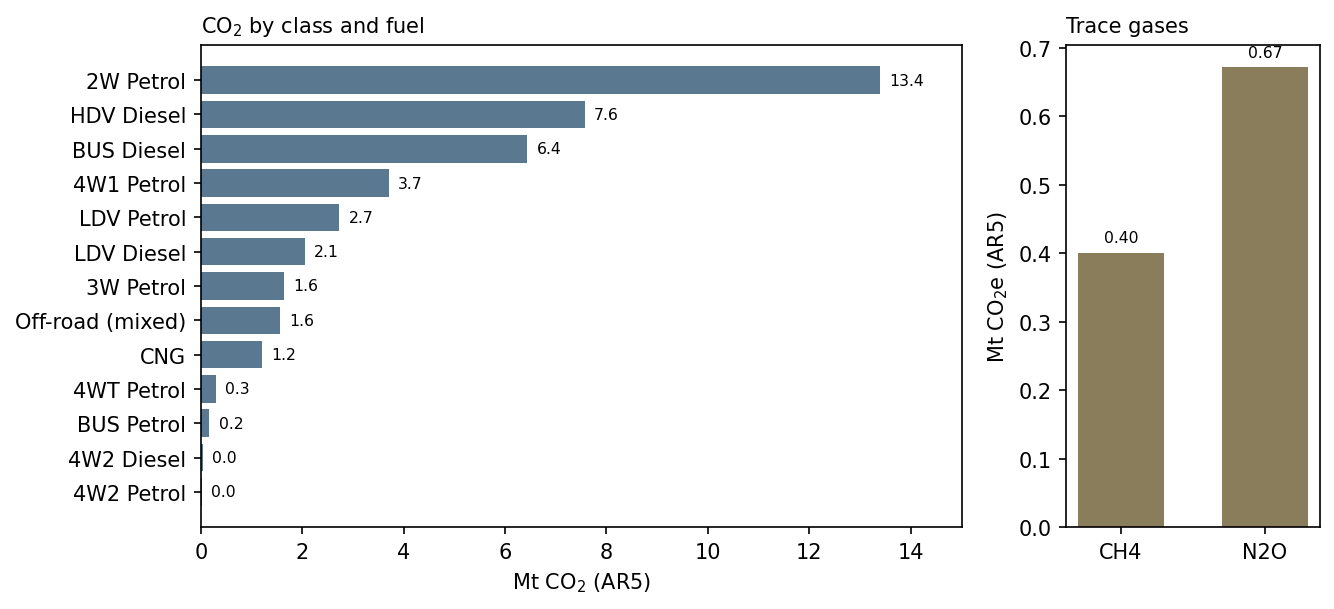
\includegraphics[width=\linewidth]{transport_composition.png}
\caption{\COtwo{} by class and fuel, with the trace gases beside on their own scale.}
\label{fig:streams}
\end{figure}

\begin{table}[htbp]
\centering
\footnotesize
\begin{tabular}{@{}lr@{}}
\toprule
\textbf{Class and fuel} & \textbf{Mt \COtwo{}} \\
\midrule
Two-wheeler petrol          & 13.395 \\
Heavy-duty diesel           &  7.578 \\
Bus diesel                  &  6.441 \\
Four-wheeler (small) petrol &  3.711 \\
Light-duty petrol           &  2.732 \\
Light-duty diesel           &  2.059 \\
Off-road machinery diesel   &  1.569 \\
Three-wheeler petrol        &  1.641 \\
CNG (all classes)           &  1.205 \\
Remaining classes           &  0.522 \\
\bottomrule
\end{tabular}
\caption{\COtwo{} by class, on the energy-weighted allocation. Two-wheelers receive
\SI{34.1}{\percent} of on-road \COtwo{}---still the largest single class, in a fleet
structure that distinguishes Pakistan from most countries whose transport inventories are
used as methodological references, but \emph{less} than heavy goods vehicles and buses
together (\SI{14.02}{\mega\tonne}). A model output, not a measured national finding, and
one this edition changed.}
\label{tab:classes}
\end{table}

\textbf{This table is where correcting the allocation showed up, and the correction
reversed its headline.} The previous edition split each fuel control by vehicle-kilometres
alone, which gives a motorcycle-kilometre the same petrol as a car-kilometre; on that
basis two-wheelers took \SI{42.3}{\percent} of on-road \COtwo{}, \SI{21.9}{\mega\tonne},
and the paper reported them as burning more than heavy goods vehicles and buses combined.
Weighting each class's kilometres by its declared energy intensity moves them to
\SI{34.1}{\percent} and \SI{13.40}{\mega\tonne}, and heavy diesel---trucks and buses at
\SI{14.02}{\mega\tonne}---becomes the larger claim on the sector. The sector total moved by
\SI{0.05}{\mega\tonne} in the process.

That is the third time in this paper's history that reading an input properly has
overturned something it previously reported, after the $\times 16/9$ control arithmetic
and the OCAC tables it described as unobtained while holding them. The pattern is worth
naming rather than quietly fixing: each correction landed in the composition or the
control provenance, never in the anchoring structure, which is the argument for the
structure. It also cuts against the convenient reading of this sector---a
two-wheeler-dominated fleet is a more novel finding than a truck-and-bus-dominated one,
and it was the artefact.

The class table remains the sector's weakest output, and the corrected version is not
better supported than the old one---it is less wrong in a knowable direction. Its three
inputs are registration counts, assumed annual kilometres and declared intensity bands,
none measured in Pakistan. What follows below prices that honestly rather than resting on
the point estimate.

\subsection{The fuel-based series the philosophy makes possible}
\label{sec:series}

The annual road-fuel series covers the same ten fiscal years as the national core, July 2015--June 2025. Fuel controls determine the total; vehicle classes provide a conditional partition. Monthly OCAC editions are held from July 2021. Earlier annual activity is allocated with explicitly weaker support and is not described as observed monthly use. Exhaust timing, evaporation and wear retain their own process evidence labels rather than inheriting one fuel profile universally.

\begin{figure}[htbp]
\centering
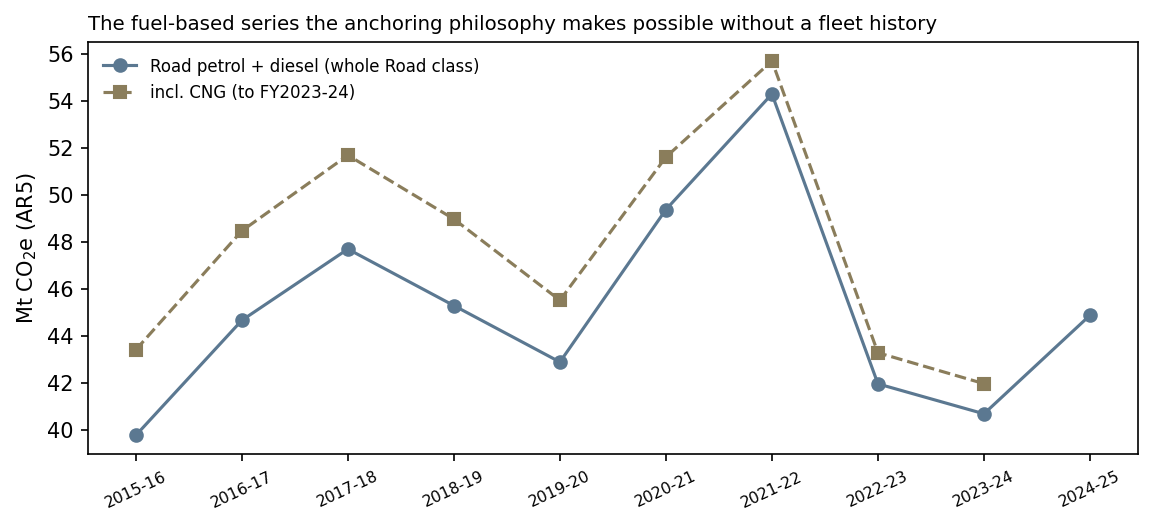
\includegraphics[width=\linewidth]{transport_fuel_series.png}
\caption{Road-class petroleum emissions, FY2015--16 to FY2024--25, with CNG added where
the OGRA series reaches (\texttt{outputs/transport\_fuel\_series.csv}). Whole-Road-class
basis, declared: no generator carve-out back-cast, no off-road partition, no class
composition. The 2022 peak and the post-2022 demand contraction are the feature EDGAR's
own series shows and a fixed-year comparison would have misread.}
\label{fig:series}
\end{figure}

The series is deliberately spartan---whole-Road-class, fuel-based, with a test asserting
its reference-year row equals the inventory's petroleum total modulo exactly the two
declared refinements---because composition over time would require the fleet history the
sector does not have, and inventing it would spend the credibility the fuel basis earns.

\subsection{Provincial allocation, now from fuel sales}

\begin{figure}[htbp]
\centering
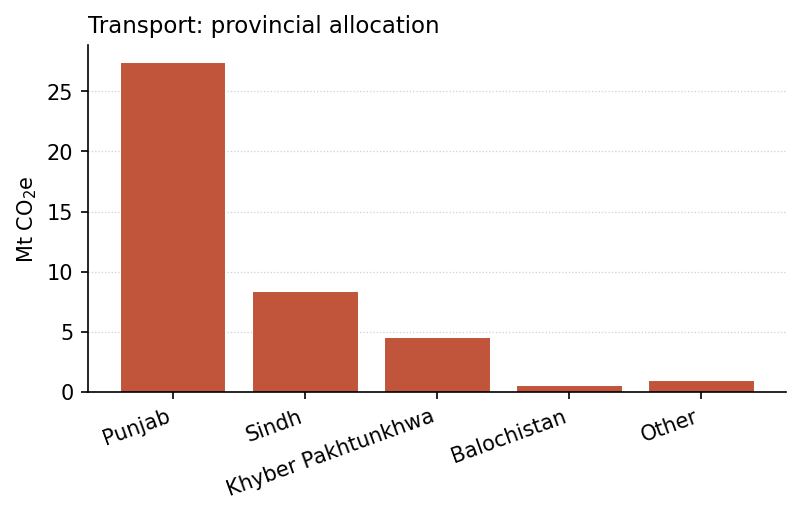
\includegraphics[width=\linewidth]{transport_provincial.png}
\caption{Punjab \SI{27.49}{\mega\tonne}, Sindh \SI{8.36}{\mega\tonne}, Khyber
Pakhtunkhwa \SI{4.52}{\mega\tonne}, Balochistan \SI{0.58}{\mega\tonne}, other
territories \SI{0.98}{\mega\tonne}. The petroleum streams ride provincial fuel sales
from OCAC's monthly area editions, per fuel; CNG and the off-road class ride their own
proxies (Table~\ref{tab:allocwalk}). Fuel sold is still not fuel consumed (freight
crosses provincial boundaries), which is the residual caveat.}
\label{fig:provincial}
\end{figure}

The petroleum streams are allocated on provincial fuel sales---the monthly area pages
of the same OCAC publication the national controls come from, summed and shared per
fuel---replacing the registration proxy whose Sindh result this paper previously
declared indefensible. The shape is the reference year's \emph{own}: twelve FY2023--24
area pages, from OCAC's direct single-month editions
(\texttt{data/activity/transport/ocac\_sectoral\_provincial.csv}).

An earlier edition of this paper borrowed FY2024--25's shape here, on the claim that OCAC
printed complete area pages ``for FY2024--25 and FY2021--22 but not for the reference
period between them''. That was true of the cumulative period-to-date editions the panel
was then built from, which carry a national page only---and false of the publication: the
direct editions of the same months carry full area pages, and the repository held all
thirty-six of them when the sentence was written. The bounding argument offered for the
borrowing was sound---the FY2021--22 bracket bounded it at \num{3.86} percentage
points---and, measured now against the reference year's own pages, the borrowed shape was
in fact off by at most \num{0.45} points on any (province, fuel) share. A sound bound
over a false premise is still not the year's own data. The neighbouring panel years
bracket the own-year shape in
\texttt{outputs/transport\_provincial\_shape\_brackets.csv}, where the largest drift
against either neighbour is \num{3.93} points---the empirical answer, kept published, to
whether borrowing a provincial shape across one year is ever defensible here. Not
every stream rides fuel sales, and Table~\ref{tab:allocwalk} says exactly which does:

\begin{table}[htbp]
\centering
\footnotesize
\begin{tabular}{@{}lll@{}}
\toprule
\textbf{Stream} & \textbf{National control} & \textbf{Provincial proxy} \\
\midrule
Road petrol   & OCAC Road MS+HOBC        & provincial petrol sales \\
Road diesel   & OCAC Road HSD, net of    & provincial HSD sales \\
              & \quad off-road partition &  \\
CNG           & OGRA national metered gas & CNG fleet energy proxy \\
Mixed off-road & HSD partition            & cropland proxy \\
\bottomrule
\end{tabular}
\caption{The allocation crosswalk: which stream rides which provincial proxy. CNG's
geography still rides the fleet model (whose CNG kilometres the two-basis check flags as
overstated), now weighted by the same declared energy intensities as the class split
rather than by distance---three-wheelers are \SI{43}{\percent} of CNG energy against
\SI{74}{\percent} of CNG distance, and the correction moves \SI{4.7}{} points out of
Punjab. The off-road class rides cropland, right for tractors and wrong for the
residual's remainder.}
\label{tab:allocwalk}
\end{table} The change is not cosmetic. Registration location gave Sindh
\SI{6.3}{\percent} of road activity, below Khyber Pakhtunkhwa, for the province
containing Karachi and the port system; fuel sales give it \SI{19.45}{\percent} of road
diesel, and diesel is allocated separately from petrol precisely because freight
geography is not passenger geography.

\begin{figure}[htbp]
\centering
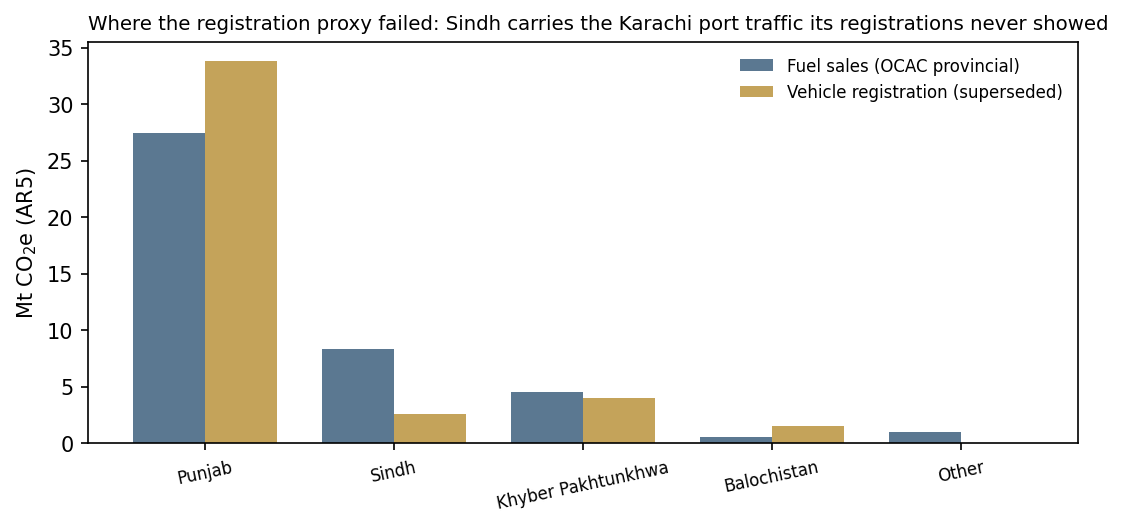
\includegraphics[width=\linewidth]{transport_provincial_proxy_gap.png}
\caption{The failure diagnostic: the superseded registration allocation against the
fuel-sales allocation
(\texttt{outputs/transport\_provincial\_proxy\_comparison\_2024.csv}). Registration
location understated Sindh by roughly a factor of three---vehicles are registered where
it is administratively convenient and fuelled where they work.}
\label{fig:proxygap}
\end{figure}

The remaining caveat is stated rather than hidden: fuel sold in a province is not fuel
consumed there, because freight transits. It is, however, the right error to be left
with---a sales-side blur on a measured quantity, rather than an administrative register
standing in for activity.

\subsection{Contribution to the national inventory}

\begin{table}[htbp]
\centering
\footnotesize
\begin{tabular}{@{}lrr@{}}
\toprule
\textbf{Category} & \textbf{Level (\%)} & \textbf{Variance (\%)} \\
\midrule
Road transport            &  9.04 & 0.90 \\
Mixed off-road (1A4c/1A2) &  0.39 & 0.01 \\
\bottomrule
\end{tabular}
\caption{Shares of the national total and of national Approach-1 variance. At IPCC category level road transportation is the
second-largest category, marginally above public electricity generation; the transport module is
the third largest category of calculation module, behind agriculture and power. It contributes
little to the uncertainty on the national total.}
\label{tab:keycat}
\end{table}

That contrast follows directly from anchoring. Road transport is \SI{9.0}{\percent} of Pakistan's emissions and
\SI{0.9}{\percent} of its inventory variance, a ratio of nearly ten to one in the
direction of "large and parametrically well constrained under the current boundary".

These are COMMON-PERIOD shares, all on FY2023--24. Measured against an FY2021--22 transport year,
the share would be \SI{12.2}{\percent}; on FY2023--24 it is \SI{9.0}{\percent}, and road transport remains
the second-largest category, only marginally above public electricity generation.

That movement is a demand history, not a methods change. Petrol sold to the Road customer
class fell from \SI{9128}{\kilo\tonne} in FY2021--22 to \SI{7209}{\kilo\tonne} in FY2023--24
and diesel from \SI{7887}{} to \SI{5551}{}, so the sector was carrying a figure from the
demand peak that preceded the post-2022 contraction while the sectors it was ranked against
had moved on two years. The previous edition predicted this: it computed the matched-year
share from the fuel series and reported it as \SI{9.43}{\percent} without adopting it. The
realised value is \SI{9.02}{\percent}, and the small remaining difference is the two
refinements the series deliberately omits---the generator carve-out and the off-road
partition.
The reason is structural: the activity datum is a metered, sold, sectorally partitioned
fuel quantity with comparatively narrow bounds, and the emissions are almost entirely
\COtwo{} from a well-characterised factor.

The practical implication is a useful negative result. Refining Pakistan's vehicle fleet model
would improve the class composition---which matters for air quality and for projecting fleet
policy---but would move the national inventory's uncertainty band hardly at all. Fleet
modelling is where transport inventory effort in developing countries usually goes, and on
this evidence it is not where the national total's uncertainty is.

\FloatBarrier
% ===========================================================================
\section{Discussion}
\label{sec:discussion}
% ===========================================================================

\subsection{What anchoring buys, and what it costs}

Anchoring gives the sector total three properties that a bottom-up estimate does not have. It
agrees with the national fuel statistics exactly rather than approximately. It is insulated
from the fleet model, so the least supported input in the sector cannot move the most used
output. And it makes the boundary problem---which customer classes are road, and what a
retail sales channel can and cannot see---visible as an executable ledger rather than
absorbed into an unexamined assumption about what fraction of diesel is "road".

The cost is real and worth naming. The class composition in Section~\ref{sec:results} is
determined entirely by the fleet model, with no independent check, so a reader wanting
emissions by vehicle type gets a number whose uncertainty this paper cannot quantify. A
bottom-up inventory would produce the same weak composition but would additionally propagate
it into the total; anchoring confines it. That is a better trade, not a free one.

There is also a subtler point, which Supplementary Note~S1 quantifies. Removing the fleet
uncertainty from the total leaves the shared fuel-carbon factor as the dominant term. An
earlier edition read the cross-sector correlation scenario as roughly doubling the band;
the common-random-numbers rebuild showed that spread to be a sampling artifact, and both
treatments of the pooled Monte Carlo now print the same $\pm\SI{12.9}{\percent}$, beside the
sector's own Approach~1 interval of $\pm\SI{11.4}{\percent}$ that the results report as the
number to quote. Anchoring does not make the
sector more certain; it makes the remaining uncertainty legible.

\subsection{What the re-anchor changed, and what it teaches}

Reading the controls from their primary table moved the sector by six megatonnes and
flipped the EDGAR comparison from above the benchmark to below it. Neither number was
the point. The previous edition's control was arithmetically inconsistent with its own
source note, and the matched-year benchmark agreement it produced was coincidence---the
wrong annualisation happened to land near the right vintage. The lesson generalises: a
benchmark comparison tests consistency, not provenance, and an inventory that treats
agreement with EDGAR as validation has its evidentiary arrow backwards.

The re-anchor also shrank the boundary problem rather than merely renaming it. Bulk
industrial, utility, government and railway diesel left the road control by the structure
of the source; what remains unresolved is the retail channel's end-use split, bounded by
the ten-year road-share panel and carried as status rows. The residual ask of Pakistani
statistics is now precise: not "publish a sectoral split"---OCAC does---but an end-use
survey of the retail diesel channel, separating road vehicles from tube wells and captive
gensets at the pump.

The asymmetry the previous edition claimed survives, strengthened: this inventory can name
what is wrong with its own transport figure more precisely than any external comparison
can. A ratio says two numbers differ; the ledger says which claimant is unresolved, in
which channel, inside which row, within what bound.

\subsection{Implications}

\textbf{Fuel controls and fleet assumptions constrain different outputs.} Fuel anchoring constrains combustion CO$_2$ and isolates the effect of class partition on that total. PM, NO$_x$, evaporation and wear remain sensitive to vehicle technologies, controls, maintenance and operating conditions. A GHG variance screen therefore cannot establish the value of fleet evidence for the air-pollutant product.

\textbf{Retail end-use evidence would constrain the source boundary.} The unresolved fraction of retail diesel used by agricultural and captive equipment affects the road/off-road assignment directly. This evidence serves a different purpose from fleet technology and vehicle-kilometre information, which constrain pollutant factors and class composition. Their value cannot be ranked using fuel-derived CO$_2$ alone.

\textbf{Two-wheelers are the largest single class, but not the largest claim.} Under the
reference allocation they receive \SI{34.1}{\percent} of on-road \COtwo{}; the
superseded run's composition envelope spanned twelve points around it, and in
every one of them heavy goods vehicles and buses together
(\SI{14.02}{\mega\tonne} at the reference) exceed them. The previous edition, splitting
fuel by distance alone, put two-wheelers at \SI{42.3}{\percent} and above heavy diesel;
that ordering was an artefact of the weighting and this edition retires it.

We draw no policy conclusion from the ordering, and the earlier draft's remark that
car-focused electrification addresses only a minority of the sector is withdrawn---not
because it is necessarily wrong, but because nothing here supports it. A ranking whose
inputs are registration counts, assumed kilometres and declared intensities, none of them
measured in Pakistan, is not a basis for allocating policy attention between vehicle
classes. What the composition can support is a weaker and more useful statement: whichever
end of the envelope holds, this is a fleet in which two-wheelers and heavy diesel each
account for a substantial share, and an inventory that resolved only one of them would
mislead.

% ===========================================================================
\section{Limitations}
\label{sec:limitations}
% ===========================================================================

\textbf{The class split has no independent validation and should be read as the sector's
weakest output.} No nationally representative Pakistani vehicle-kilometre survey has been
identified for this study, and no on-road fuel-economy measurement either. The shares rest
on three inputs, none of them measured in the country: registration counts, assumed annual
kilometres, and the declared per-kilometre energy intensities that weight them. The largest
single result---two-wheelers at \SI{34.1}{\percent} of on-road \COtwo{} under the
reference allocation---rests on the least surveyed class in the fleet and on a judgement about how
much fuel a motorcycle burns.

This edition changed that result, which is itself a limitation worth stating: the previous
allocation weighted kilometres alone and put two-wheelers at \SI{42.3}{\percent}, above
heavy goods vehicles and buses combined. Correcting the weighting reversed that ordering.
A reader should conclude that the composition is not yet settled, not that it is now
settled differently. Anchoring confines the consequence to composition rather than total,
which is the reason the method was chosen, but it does not make the composition reliable.

\textbf{The off-road class is a residual as well as a category, and part of it belongs to a
different IPCC code.} The source workbook maps its catch-all "other vehicles" entry into
off-road wholesale, and the whole class is then modelled as \SI{100}{\percent} diesel. The
magnitude of the carve-out is therefore a genuine partition of the fuel total, while what
is inside it is soft. Whatever construction and industrial machinery the residual contains
belongs under 1A2\,gvii, not 1A4c; this inventory reports the whole class under the
mixture-declaring name \emph{Mixed off-road (1A4c/1A2)}, declares the misassignment in the
completeness table, and prices the reporting recode as a scenario, because splitting the
residual needs equipment stock data no source here provides. The cropland proxy that
allocates it provincially is right for tractors and wrong for whatever else the residual
contains.

\textbf{Retail-bought agricultural and captive diesel remain inside the road residual.}
Tube wells, threshers and captive generators fuelled at retail pumps draw on the Road
customer class, this inventory has not separated them, and they bias the road residual
high---conditional on the other deductions, since errors in the generator carve-out or
the off-road partition could run either way. The claim is framed rather than open-ended:
bulk agricultural HSD is observed zero in all ten OCAC editions; the ten-year road
share of national diesel (0.83--0.91) is a customer-class boundary sensitivity that
bounds the sales channel, not the contamination within it; and the retail non-road
scenarios price the within-channel claim at 2.5--10\% of the Road row
(Table~\ref{tab:boundary}). Resolving it needs a retail-channel end-use survey, which no
identified source provides. The ledger carries three claimants as \textsc{unresolved}
status rows---the third, "other retail stationary/non-road uses", because the named two
are not proven exhaustive.

\textbf{The provincial allocation now rides fuel sales, whose residual blur is transit.}
Fuel sold in a province is not fuel consumed there---freight crosses provincial
boundaries, so Sindh's \SI{19.45}{\percent} of road diesel partly reflects fuel bought at
Karachi and burned en route north. The shape is the reference year's own twelve area
pages---an earlier edition borrowed FY2024--25's here on the false premise that none were
published for the reference period, a borrowing since measured at no more than \num{0.45}
percentage points of error on any share. This is a far smaller distortion than the superseded
registration proxy's (which understated Sindh threefold; the comparison is published as a
diagnostic), but it is a real one. The release now ships the road geometry that a finer
allocation would start from---\texttt{outputs/pakemis\_road\_length\_adm2.csv} and a
\SI{0.05}{\degree} major-road density raster, extracted from a dated, hashed OSM
snapshot---as a diagnostic only: road length is not traffic, and moving fuel onto the
network would need traffic observations this inventory does not hold. CNG's provincial split still rides the fleet
model and the off-road class rides cropland (Table~\ref{tab:allocwalk}); only the
petroleum streams ride fuel sales.

\textbf{The CNG heating value is unpinned.} CNG is estimated from OGRA's metered sector
gas, but OGRA reports a volume and IPCC works in net terajoules: the conversion applies a
gross heating value and then the \num{0.90} gross-to-net factor for natural gas. The
gross-to-net step is a documented convention; the gross value is not---Pakistani pipeline gas
runs \SIrange{900}{1000}{} Btu/scf depending on field and RLNG share and nothing read here
pins it. Both ends are reported; the span is \SI{0.13}{\mega\tonne}, a tenth of the CNG
stream. This is the same unresolved quantity as the captive-power category's heating value,
and the two sectors are pinned to the same values by test so that one inventory cannot
assume the same gas two ways.

\textbf{The fleet model overstates CNG travel, and this sector has evidence rather than a
suspicion.} Section~\ref{sec:validation} divides the metered gas by the modelled CNG
vehicle-kilometres and gets \SI{0.91}{\mega\joule\per\kilo\metre}, below any plausible
value for a fleet seven-tenths three-wheelers by distance. The consequence is confined to
what rides vehicle-kilometres---the air diagnostic and the CNG streams' provincial
split---because the CNG emissions come from metered gas. It is nonetheless the clearest
evidence in this paper for the sector's central methodological choice.

\textbf{The air layer is an exploratory diagnostic, on factors without provenance.} The
per-kilometre factors are transcriptions of the Punjab emissions workbook, for which no
primary citation has been located---an earlier draft attributed them to the EMEP/EEA
guidebook, whose road-transport chapter has not in fact been acquired here. Evaporative
NMVOC and non-exhaust particulate are not estimated at all (both are named process
families in the gap register with the public chapters that would supply them), and
\SOtwo{} scales with an unreported fuel sulphur content. The layer is accordingly
reported in an appendix with no policy claims built on it.

\textbf{The time series is fuel-only, by design.} The ten-year fuel series
(Section~\ref{sec:series}) carries no generator back-cast, no off-road partition and no
class composition, because the inputs those refinements need exist only for the reference
year. The declared whole-Road-class basis keeps the series honest; it also means the
series is a magnitude record, not a structural one.

\textbf{Emission factors are Tier~1 defaults throughout.} They carry assumptions about
technology mix and combustion conditions derived largely from countries whose vehicle fleets
differ substantially from Pakistan's---most consequentially for the two-wheeler class, which
dominates here and is marginal in the fleets the defaults were derived from.

\textbf{The controls are member-supplied.} OCAC's own disclaimer states its data are
provided by members and not independently verified. The declared \SI{10}{\percent}
control uncertainty is anchored on the independent cross-check available---the railway
figures, \SI{3.8}{\percent} apart year-matched and \SI{11.2}{\percent} on the
conservative cross-year pairing---and the panel's internal closures, and it is a
judgement, not a fit.

% ===========================================================================
\section{Conclusion}
\label{sec:conclusion}
% ===========================================================================

Pakistan's road transport---the conditional road residual under the current claimant
assignment---emitted \SI{40.19}{\mega\tonne} \COe{} in FY2023--24 and its mixed off-road
machinery \SI{1.73}{\mega\tonne}, together \SI{9.4}{\percent} of a ten-sector national
inventory in which all ten sectors now report the same twelve months. Both are
anchored on the road customer class of the national sectoral sales table, plus metered
transport CNG, so the sector total agrees with Pakistan's fuel statistics by construction
rather than by adjustment.

Three results generalise beyond this country.

\textbf{Anchoring puts the weakest input where it does least damage.} A fleet model that
distributes a known quantity of fuel cannot move the sector total; one that sizes it can. The
class composition reported here is no better supported than any bottom-up equivalent---worse,
in a country with no identified vehicle-kilometre survey---but it is confined to the output
where its weakness matters least. The arrangement is what the IPCC guidance implies where fuel
statistics are strong and fleet data weak, and it is rarely stated as a design choice.

\textbf{A customer-class table is a claimant ledger waiting to be read.} Pakistan's
sectoral sales statistics partition national fuel exhaustively---road, rail, navigation,
power, industry, government---and reading the partition into a two-tier ledger replaced
most of a boundary argument with observation: bulk claimants excluded by the source's own
structure, one carve-out relayed from the sector that measures it, one partition, an
independent cross-check where two unrelated sources report the same boundary row, and the
genuinely unresolved remainder---the retail channel's end-use split---carried as priced
status rows, because naming a residual's direction and sensitivity is more useful than a
correction nobody can evidence.

\textbf{A benchmark match is not provenance.} The previous edition's control total was
arithmetically inconsistent with its own source note, and a matched-year EDGAR comparison
failed to notice, because the wrong number landed near the right vintage. Correcting the
provenance moved the sector six megatonnes and flipped the comparison's direction; on a
scope inferred from EDGAR's category-resolved source files and a fiscal-year-blended
benchmark on the reference period the estimate now sits at \num{0.85} of the blend---a
scope-approximate diagnostic, with the rc4-era \num{0.70} retained in the comparison
table as a superseded mixed-vintage construction. The
paper retains the superseded control as a named executable scenario---the bridge readers
of the earlier edition are owed---and draws the general moral: external agreement tests
consistency, and only provenance tests provenance. The parallel-table \NtwoO{} trap
(Section~\ref{sec:factors}) makes the same point from the factor side: a
\COtwo{}-dominated validation cannot detect a category running \SI{8}{\percent} low
through the wrong trace-gas table.

Fuel controls constrain the GHG magnitude, while end-use claimant evidence constrains the road/off-road boundary. Fleet technologies and operation remain consequential for pollutant factors even when class shares have little effect on fuel-derived CO$_2$. The annual national core covers July 2015--June 2025; the detailed reference-year class analysis does not constitute observed historical fleet composition.

Archived input tables, source-factor registers, build commands, plotted data and numerical checks accompany the sector estimates. The release distinguishes regeneration from compiled tables from a full primary-source extraction.

\FloatBarrier

% ---------------------------------------------------------------------------
\section*{Code and data availability}
% ---------------------------------------------------------------------------

The calculation engine, the activity data, the fleet model and every output quoted here
are version-controlled in the inventory repository
(\url{https://github.com/RehanAhmad13/pakistan-emissions-sectors}); an archived release
with a Zenodo DOI is minted at submission. The sector is regenerated with
\texttt{python3 -m pkinv.sectors.transport.run\_transport}, which requires the railways
and residential modules to be importable for the boundary relays; \ref{app:repro} gives
the full sequence, and the run manifest hashes every primary source. Not every input
source is independently published: the archived input package ships the internal Punjab
transport manuscript and cached source extracts, and the per-kilometre air factors carry
no located primary citation and are labelled as such wherever they appear. Every number
printed in this paper is read from a generated CSV rather than transcribed, and a test
asserts that the manuscript and the engine agree.

% ---------------------------------------------------------------------------
\bibliographystyle{elsarticle-harv}
\bibliography{../../paper_common/references}

% ---------------------------------------------------------------------------
\appendix
\renewcommand{\thetable}{\arabic{table}}%
\renewcommand{\thefigure}{\arabic{figure}}%
% ===========================================================================
\section{Reproduction}
\label{app:repro}
% ===========================================================================

The sector runs on Python 3.11 with no compiled dependencies:

{\footnotesize
\begin{verbatim}
pip install -e .
python3 -m pkinv.sectors.transport.run_transport
python3 -m pkinv.sectors.transport.air_pollutants
\end{verbatim}
}

which writes \texttt{transport\_totals\_2024.csv},
\texttt{transport\_by\_stream\_2024.csv}, \texttt{transport\_fuel\_2024.csv},
\texttt{transport\_provincial\_2024.csv},
\texttt{transport\_air\_pollutants\_2024.csv}, the twelve-month layer
(\texttt{transport\_\allowbreak monthly\_\allowbreak 2024.csv}, each month's share with the emissions it implies
and the basis of the shape), the two-tier fuel-claimant ledger
(\texttt{transport\_fuel\_ledger\_2024.csv}), the uncertainty system
(\texttt{transport\_uncertainty\_2024.csv} and its variance-decomposition, inputs-register
and structural-scenario companions), the ten-year fuel series
(\texttt{transport\_fuel\_series.csv}), the provincial proxy comparison
(\texttt{transport\_provincial\_proxy\_comparison\_2024.csv}), the mass-to-energy fuel
bridge (\texttt{transport\_fuel\_bridge\_2024.csv}), the OCAC consistency diagnostic
(\texttt{transport\_ocac\_control\_diagnostic.csv}) and a run manifest
(\texttt{transport\_run\_manifest\_2024.json}) that hashes every primary source---
including all 57 OCAC sectoral PDFs---to \texttt{outputs/}.

The OCAC sectoral CSVs the controls read are committed data; regenerating them from the
PDFs is a separate, deterministic step
(\texttt{python3 scripts/ingest\_ocac\_sectoral.py}, requiring \texttt{pdftotext}), and
an ingest test pins the committed cells to independently verified values.

The relays are not constants in this sector. Household-generator petrol is read from the
residential module (a carve-out) and railway diesel from the railways module (a
cross-check), so reproducing the boundary requires both to be importable:

\begin{verbatim}
python3 -c "\
from pkinv.sectors.residential import combustion
print(combustion.generator_petrol_kt())"
python3 -c "\
from pkinv.sectors.railways import traction
from pkinv.sectors.railways import data as rw
print(traction.diesel_kt(rw.RailwaysData()))"
\end{verbatim}

Figures are regenerated with \texttt{python3 -m pkinv.report.figures} and copied into this
manuscript by \texttt{python3 scripts/sync\_figures.py}; a test fails if any shipped figure
differs from the output it plots. The full suite runs with
\texttt{python3 -m unittest discover tests}.

% ===========================================================================
\section{Sources}
\label{app:sources}
% ===========================================================================

Fuel controls are the Road customer-class rows of OCAC's Sectoral Sales of Energy
Products, annual and monthly-provincial editions \citep{ocacarchive}, with the superseded
Economic Survey-derived pair \citep{econsurvey2025energy} retained as a scenario;
transport CNG is OGRA's sectoral gas statistics \citep{ogra2024,ograarchive}, with the
billing heating-value basis from the two gas utilities \citep{sngpl2024,ssgc2024}.
Vehicle counts by class and province come from the provincial registration tables
\citep{provregstats}. The Weibull survival parameters and the per-class MJ/km intensity
bands are in \texttt{data/transport\_params.csv} with a source string on every row---the
survival parameters from the Punjab district-level transport manuscript
\citep{naveedpunjab}, which adopts \citet{guttikunda2024}; the intensity bands are this
inventory's own declared engineering judgement and say so. The annual kilometres and fuel
splits are separate tables (\texttt{data/activity/transport/vkt.csv},
\texttt{fuel\_split.csv}), transcribed from the same manuscript's workbook, which carries
no per-row citation for them; they are declared without primary provenance in their own
source columns and registered as a gap
(\texttt{transport-class-activity-provenance}). A previous edition of this appendix said
all three lived in the parameter table with sources recorded per row, which was not true
of two of them. The rail cross-check reads the
Pakistan Railways Year Book \citep{pakrailyearbook2024} through the railways module; the
generator carve-out reads HIES \citep{hies2025} over the administered petrol price
\citep{goppetrol} through the residential module. Emission factors are
IPCC 2006 Guidelines Volume~2 Chapter~3 defaults \citep{ipcc2006energy}: Table~3.2.2 for
road, Table~3.3.1 for off-road machinery. Air factors come from held EMEP/EEA 2023 source chapters, with separate fuel, evaporation and wear units and an explicit class/fuel bridge (Section~\ref{sec:air}). Supplementary Note~S2 renders the current source tables and clearly labels the superseded diagnostic rows as historical. External
comparison is EDGAR's series \citep{edgar2025booklet}, read at this sector's fiscal
year as a blend of the 2023 and 2024 columns (\SI{48.13}{\mega\tonne}); the
CY2021/CY2022 blend survives only as the superseded rc4 construction in the
comparison table.

Every factor in the repository carries a source string, and a provenance test asserts that
none is empty and that any informally sourced value is declared as such. The declared MJ/km intensity bands remain engineering assumptions rather than Pakistani operating measurements. Source-based air factors likewise require an applicability assessment for the transferred fleet and fuel technology. A source string is not the same thing as a citation, and the distinction
is made explicit rather than averaged away.

% ===========================================================================
\section{Supplementary Note: why the shares are normalised over all classes}
\label{app:shares}
% ===========================================================================

The off-road class is included in the denominator that normalises the vehicle-kilometre
shares, and removing it is a mistake worth documenting because it is the natural thing to try.

Suppose off-road were dropped from the fleet before normalising, on the reasoning that this
sector reports road transport. The remaining classes' shares would then sum to one over the
\emph{whole} diesel supply, so on-road vehicles would be assigned \SI{100}{\percent} of the
national diesel. Any separate estimate of off-road machinery---whether made here, in another
sector, or by another author---would then claim its fuel a second time. The national diesel
figure would support more emissions than there is diesel.

Keeping off-road inside the normalisation makes the two categories an exhaustive partition of
one fuel quantity: their shares sum to one, so their emissions sum to the control total times
the factor. The memo item that formerly carried off-road as a \COtwo{}-only note outside all
totals is asserted to be empty, which is the test that catches a future edit reintroducing the
double count.

The same structure appears in this inventory's waste sector, where one municipal waste
generation figure is partitioned between disposal and open burning
\citep{ahmad2026national}. In both cases the useful property is not that the split is right,
but that an argument about the split cannot change how much of the underlying quantity exists.

\FloatBarrier
% ===========================================================================
\section{Supplementary Note: Road-Transport Air Pollutants (EMEP/EEA Tier~1)}
\label{sec:air}
% ===========================================================================

This note reports the FY2023--24 road air-pollutant estimate using the EMEP/EEA 2023 Tier~1 factors. Native pollutant masses remain separate from greenhouse-gas aggregates. The national release extends the same source methods through FY2024--25 with source-year activities and declared factor applicability.

\textbf{Fuel is the activity, and it reconciles to the controls by construction.}
Tier~1 exhaust factors are grams per kilogram of fuel; the fuel each vehicle class
burns is the OCAC Road control total for the year---the same panel the greenhouse-gas
side burns, net of the same household-generator carve-out---split between classes by
the fleet model's energy-weighted class shares. Modelled fuel therefore equals sold
fuel for every fuel in every year, the anchor the superseded diagnostic explicitly
lacked; the class \emph{split} still rides the fleet model, so composition remains the
sector's weakest axis while the fuel quantity is constrained. Four process families are
estimated as separate atoms: hot-plus-cold exhaust (fuel-based), evaporative petrol
NMVOC (per-vehicle-day, at the guidebook's 20--35\,\si{\celsius} daily temperature
range, on the fleet model's own active vehicle counts), and tyre-and-brake and
road-surface wear (per vehicle-kilometre). Black carbon is the guidebook's f-BC
fraction of exhaust \PM{}---a component of particulate mass, never additional---and
\SOtwo{} is sulfur stoichiometry under the declared per-year fuel-sulfur regime of
\texttt{data/activity/transport/fuel\_sulfur\_by\_year.csv} (diesel on the same cited
Euro-II/Euro-V mandate boundaries the railways layer burns). Where the guidebook
publishes no Tier~1 factor for a Pakistani cell, the bridge table
(\texttt{data/activity/transport/emep\_class\_map.csv}) declares a named proxy---light
CNG vehicles take the passenger-car LPG chemistry, petrol buses the light-commercial
petrol row---never a silent one.

\begin{table}[htbp]
\centering
\footnotesize
\begin{tabular}{@{}lr@{}}
\toprule
\textbf{Pollutant} & \textbf{Tier~1 (kt/yr)} \\
\midrule
CO                   & 1430.4 \\
NMVOC                &  535.1 \\
\NOx{}               &  172.1 \\
\SOtwo{}             &   12.2 \\
\PM{}                &    8.2 \\
Black carbon         &    2.0 \\
\NHthree{}           &    2.6 \\
\bottomrule
\end{tabular}
\caption{Road transport, FY2023--24, EMEP/EEA Tier~1 on OCAC-reconciled fuel, all
processes. NMVOC is non-methane VOC;
\NOx{} is NO$_2$-equivalent mass, the inventory-wide basis. \PM{} here is the PM$_{2.5}$
core (exhaust \PM{} is PM$_{2.5}$ by the chapter's own statement, plus the wear
processes' PM$_{2.5}$); the wear processes' coarser TSP and PM$_{10}$ strata are
supplemental beside it, contained not additive, and appear in the factor appendix. The native factor definitions remain documented by process.}
\label{tab:air}
\end{table}

\begin{figure}[htbp]
\centering
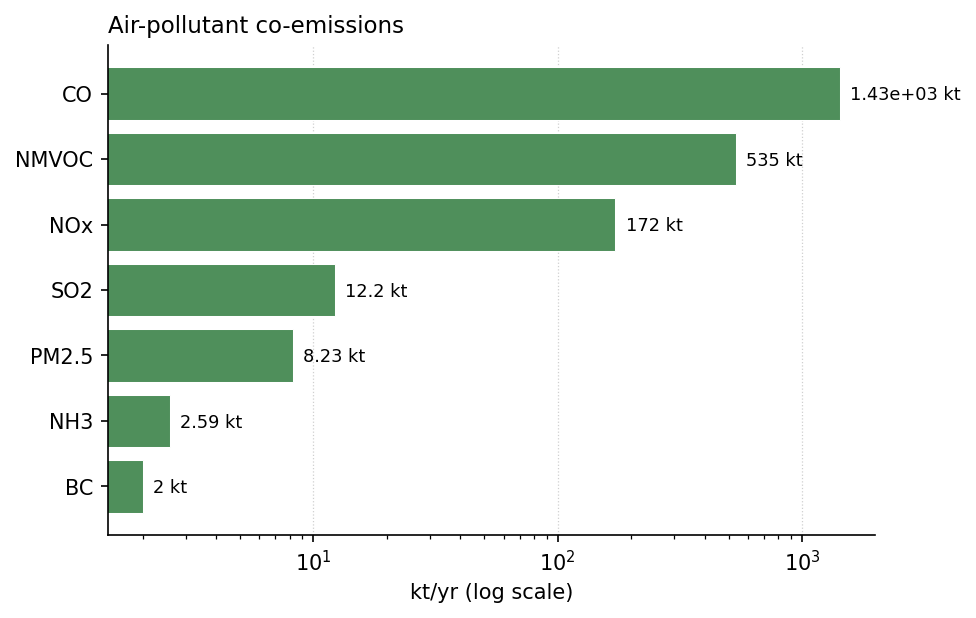
\includegraphics[width=\linewidth]{transport_air.png}
\caption{The Tier~1 layer, log axis: carbon monoxide exceeds black carbon by nearly
three orders of magnitude, which a linear axis cannot show. Wear TSP and PM$_{10}$
are excluded from the bars for the same containment reason the residential figure
excludes them.}
\label{fig:air}
\end{figure}

\subsection{Interpretation and conditional uncertainty}

A fuel balance constrains the amount consumed, but does not validate a transferred PM or NO$_x$ factor. Tier~1 fleet averages describe the guidebook's reference technologies and operating conditions; Pakistan's vehicle ages, two-wheelers, maintenance, catalysts and duty cycles remain unresolved. The source min--max factor spans and explicit technology cases therefore describe consequential assumptions rather than observed national fleet confidence limits. CNG-to-LPG chemistry and the petrol-bus class substitution remain named proxies. The conditional parameter ensemble retains its declared factor widths; separate technology and sulfur endpoints receive no assigned probability.

Exhaust, evaporation and wear retain distinct process records. Fuel-sales months support exhaust timing only as a combustion proxy. Evaporation and wear lack own-year monthly process evidence and use explicitly weaker allocation. Sulfur policy dates establish the specification scenario, not universal pump-level compliance. Primary particulate mass is an emission quantity; it does not provide ambient concentration, exposure or a health ranking.

\subsection{Limitations of this layer}

Tier~1 resolves fuel and broad vehicle category, not technology vintage, catalyst
penetration or after-treatment; the class split rides the fleet model's declared
intensity weights; the fuel-sulfur regime is declared from the import-mandate record,
not measured at the pump, and domestic-refinery waivers mean the post-2021 central
deliberately stays at the conservative pre-Euro-V specification; evaporative factors
assume the guidebook's hottest daily temperature band year-round; road-dust
resuspension stays out until a defensible local silt basis exists---a different claim,
recorded in the gap register to stop it riding in.

\FloatBarrier

\end{document}
